%!TEX root = ../thesis.tex
% NIR-information

\chapter{Information content in the \nir{}}
\label{cha:nir_content}

The work presented in this chapter focuses on calculating and analysing the information content of stellar spectra, specifically the radial velocity {RV} precision of M-dwarf spectra in the \nir{}. 
M-dwarfs are a source of focus in the community with several new instruments dedicated specifically to detecting planet around M-dwarfs~\citep[e.g.][among others]{quirrenbach_carmenes_2014, bouchy_nearinfrared_2017, artigau_spirou_2014}.
The fundamental radial velocity precision of {M-dwarf} spectra attainable at different wavelength regions calculated in~\citet{figueira_radial_2016} was used to inform some design choices of two \nir{} spectrographs, {SPIRou} and {NIRPS}.
Understanding the underlying precision of different spectral types can also allow {RV} surveys to adjust the focus of the target selection, or optimize the exposure time of different spectral types.
This can help in detecting the presence of ``habitable Earth-like'' planets around {M-dwarfs} which have become a prime target with the recent \nir{} spectrographs.

The purpose of the work presented in this chapter is to extend the work of~\citet{figueira_radial_2016}, computing the theoretical {RV} precision of synthetic stellar spectra over a wider range of situations.
A investigation into the effect of \Logg{} and \feh{} on precision is performed and a preliminary comparison of {RV} precision of the recently observed \nir{} {M-dwarf} spectra from {CARMENES} library and their synthetic counterparts is given.
This is to test how the {RV} precision of synthetic models compares to reality.
New computations of the {RV} precision of synthetic spectral libraries are also given, which were provided for exposure time calculators of {NIRPS} and {SPIRou}.


\section{Overview}
\label{sec:precision_overview}
The pursuit of detecting exoplanets, especially ``habitable'' and ``Earth-like'' planets, requires state-of-the-art instrumentation with high precision.
Several new high-resolution \nir{} spectrographs are becoming available now and in the near future, not limited to {CARMENES}, {NIRPS}, {SPIRou} and {CRIRES+} (see \cref{subsec:new_generation}).
One science objective common to all four instruments is the detection of small mass planets around {M-dwarf} stars utilizing the radial velocity technique, an objective strived for in the literature~\citep[e.g.][]{reiners_detecting_2010, rodler_detecting_2011, plavchan_radial_2015}.
As the {RV} amplitude is \(\kone\propto {P}^{-{1/2}}{\mone}^{-2/3}\) (\cref{eqn:k_relation}), the induced {RV} wobble from a similarly massive exoplanet is larger around an M-dwarf star, making the {RV} signal from lower mass exoplanets easier to detect.
Also the cooler {M-dwarfs} have habitable zones closer to the star, at shorter orbital periods, that again have a stronger {RV} amplitude making it easier to detect small mass planets in the habitable zone of {M-Dwarfs}.

To calculate and predict the information content attainable from {M-dwarfs} in the \nir{,}~\citet{figueira_radial_2016} utilized the {PHOENIX-ACES} library of synthetic spectra.
This helped at the early stages of instrument design by identifying the wavelength regions with the best {RV} precision, but can also help in the planning of observations, by understanding how the precision changes with spectral type and observed {\snr{}}.
However, the synthetic spectra do not quite match reality and a comparison between theoretical and observed is needed.
\citet{artigau_optical_2018} recently compared optical ({HARPS}, {ESpaDOnS}) and \nir{} ({CRIRES}) archival spectra of the {M-dwarf}, Barnard's Star, to synthetic spectra.
They found that state-of-the-art atmosphere models over-predict the {RV} content \emph{Y}- and \emph{J}-band {RV} by more than a factor of \(\sim\)2, while under-predicting the \emph{H}- and \emph{K}-band content by half.
A similar comparison will be made in this work to {CARMENES} spectra.

Recent results regarding the measured performance of the {CARMENES} survey~\citep{reiners_carmenes_2018,quirrenbach_carmenes_2018} find that the {RV} in the \nir{} is worse than the pre-survey predictions.
Precisions of 1--2\mps{} have been achieved in the optical but only 5--10\mps{} in the \nir{}.
However, comparing {RV} precision in different wavelength bands~\citet{quirrenbach_carmenes_2018} found a ``sweet spot'' around 0.7--0.8\um{} with deep \ce{TiO} bands providing rich {RV} information in mid-M dwarfs.

The number of papers on this thematic, the number of open questions, and the impact on the design of instrumentation, particularly in the \nir{}, show that this is an important topic as of today.
  

%!TEX root = ../../thesis.tex


\subsection{Fundamental photon noise limitation}
\label{subsec:fundamental_precision}
A technique to calculate the theoretical radial velocity precision of a spectrum using the full spectral information in an optimal way was first presented by~\citet{connes_absolute_1985}.
Here the radial velocity precision derivation following~\citet{connes_absolute_1985, bouchy_fundamental_2001, figueira_radial_2016} is provided.

\begin{figure}
    \centering
    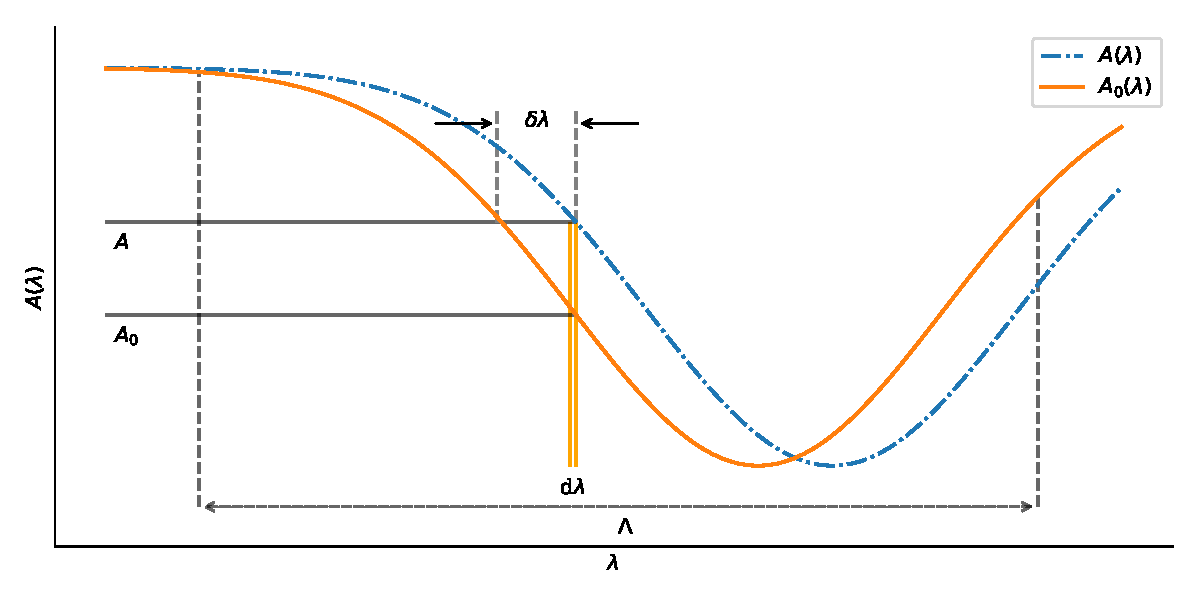
\includegraphics[width=0.8\linewidth]{figures/information-content/precision_plot.pdf}
    \caption[Demonstration of a shifted arbitrary spectral line.]{Arbitrary spectral line with a shift \(\delta \lambda\), inspired by~\citet{connes_absolute_1985}.
        \(\Lambda\) is the wavelength range considered.}
    \label{fig:precisionderivation}
\end{figure}
\todo{add \(\delta A\) to plots}

For demonstration purposes \cref{fig:precisionderivation} shows a portion of an arbitrary spectrum \(A(\lambda)\), for demonstration purposes over a wavelength range \(\Lambda\).
Here \({A}_{0}(\lambda)\) is the reference spectrum while \(A(\lambda)\) is observed some later time with an apparent wavelength shift observed.
The majority of a single Gaussian line is shown as spectral lines contain the most information but the presence of spectral lines is not a requirement for the derivation.

The Doppler shift of a spectrum is given by:
\begin{equation}
\frac{\delta V}{c} = \frac{\delta \lambda}{\lambda},
\label{eqn:dopplershift}
\end{equation}
where \(c\) is the speed of light in a vacuum, and \(\delta \lambda\) is the shift in wavelength \(\lambda\) due to the velocity \(\delta V\).

\todo{intensity change from connes is vertically in the slice d lambda}

Using basic calculus \(\delta y = \pd{y}{x} \delta x \nonumber\), and for a Doppler shift that is small compared to the line-width\footnote{Although~\citet{connes_absolute_1985} show that the approximation in \cref{eqn:intensitychange} is adequate under all circumstances.}, the observable intensity change in a wavelength slice \(d \lambda\) (or at a given pixel) can be expressed by:
\begin{equation}
\delta A(i) = A(i) - {A}_{0}(i) \simeq \pd{{A}_{0}(i)}{\lambda(i)} \delta \lambda = \pd{{A}_{0}(i)}{\lambda(i)} \frac{\delta V(i)}{c}\lambda(i).
\label{eqn:intensitychange}
\end{equation}

Rearranging \cref{eqn:intensitychange} for \(\delta \lambda\) and combining it with \cref{eqn:dopplershift}, the Doppler shift then becomes:
\begin{equation}
\frac{\delta V(i)}{c} = \frac{A(i) - {A}_{0}(i) }{\lambda(i) (\partial {A}_{0}(i)/\partial \lambda(i))} \label{eqn:delta_v_i}
\end{equation}

This equation shows that the radial velocity measured at pixel {\(i\)}, through a change in the intensity in the recorded spectrum, \(A(i)-{A}_{0}(i)\), and inversely proportional to the slope of the spectrum, \({\partial {A}_{0}(i)}/{\partial \lambda(i)}\).
\Cref{eqn:delta_v_i} provides a separate measurement of the radial velocity shift for every pixel, \(i\), in the spectrum.
The sensitivity of the velocity measurement can be improved, and the noise decreased by using the information from the whole spectral range, \(\Lambda\).
This is achieved by taking the weighted average\footnote{Weighted average on x is \(\bar{x} = \frac{\sum{ x(i)W(i)}}{\sum {W(i)}}\)} over all pixels in the spectral range using an optimal pixel weight \(W(i)\).

\begin{equation}
\overline{\frac{\delta V}{c}} = \frac{\sum{\frac{\delta V(i)}{c}W(i)}}{\sum {W(i)}}.
\end{equation}

Statistically, the optimal weights are proportional to the inverse square of the individual dispersion (variance),
\begin{equation}
W(i) = \frac{1}{{\left(\frac{\delta V_{\rms}(i)}{c}\right)}^{2}}, \label{eqn:weights}
\end{equation}
where \(X_{\rms}\) is the dispersion on the quantity \(X\).

The individual dispersion of the velocity measurement \(\delta V_{\rms}(i)\) is the dispersion that would result from several measurements of the reference spectrum all with the same Doppler shift (e.g.\ zero).
\Cref{eqn:delta_v_i} thus becomes:
\begin{equation}
\frac{\delta V_{\rms}(i)}{c} = \frac{{[A(i) - {A}_{0}(i)]}_{\rms} }{\lambda(i) (\partial {A}_{0}(i)/\partial \lambda(i))}.
\label{eqn:delta_v_i_rms}
\end{equation}
The noise of the spectrum \(A\) is the quadratic sum of the photon noise \(\sqrt{A}\) and the detector noise \({\sigma}_{D}\).
The spectrum \({A}_{0}\) is considered noise free.

\begin{equation}
{[{A(i)-{A}_{0}(i)}]}_{\rms} = {[{A(i)} - 0]}_{\rms} = \sqrt{{\sqrt{A(i)}}^{2} + {{\sigma}^{2}}_{D}} \label{eqn:noise}
\end{equation}

Considering that the Doppler shift is small and that \(A\) and \({A}_{0}\) have the same intensity level, then \(A = {A}_{0}\) can be set.
Using \cref{eqn:delta_v_i,eqn:weights,eqn:noise} the optimum weights then become solely dependent on the reference spectrum.

\begin{equation}
W(i) = \frac{{\lambda}^{2}(i) {({\partial {A}_{0}(i)}/{\partial \lambda(i)})}^{2}}{A_0(i) + {\sigma}^{2}_{D}} \label{eqn:optimal_weight}
\end{equation}

This weighting function can be modified to mask out and eliminate unwanted lines in the spectrum (see \cref{subsec:masking_function}).
For instance setting the particular pixel weights to zero to remove any telluric absorption lines in the observed spectra.

With the optimal weights set, the weighed average velocity change measured from the full spectral range \(\Lambda\), is given by:

\begin{align}
\frac{\overline{\delta V}}{c} &= \frac{
    \sum{
        \frac
        {A(i) - {A}_{0}(i)}{
            \lambda(i) \left({\partial {A}_{0}(i)}/{\partial \lambda(i)}\right)} W(i)}
}
{\sum{{W(i)}}} \\
&= \frac{
    \sum {
        \frac
        {A(i) - {A}_{0}(i)}
        {\lambda(i) (\partial {A}_{0}(i)/\partial \lambda(i))}
        \frac
        {{\lambda}^{2}(i) {({\partial {A}_{0}(i)}/{\partial \lambda(i)})}^{2}}
        {A_{0}(i) + {\sigma}^{2}_{D}}
    }
}
{\sum{{W(i)}}} \\
&= \frac{
    \sum { 
        (A(i) - {A}_{0}(i))
        \frac
        {\lambda(i) {\partial {A}_{0}(i)}/{\partial \lambda(i)}}
        {A_{0}(i) + {\sigma}^{2}_{D}}
    }
}
{\sum{{W(i)}}} \\
&= \frac{\sum{(A(i) - {A}_{0}(i)){\left(\frac{W(i)}{{A}_{0}(i) +{\sigma}_{D}^{2}}\right)}^{1/2}}}{\sum{W(i)}}
\label{eqn:delta_v_eqarray}
\end{align}

The important quantity for {RV} measurements is not just the velocity values themselves but also the dispersion (or uncertainty) on the measured velocity, the {RV} precision \(\delta V_{\rms}\), from the spectrum.
This allows one to assess the planetary detectability limitations attainable in the spectra.
From rearranging \cref{eqn:weights} the dispersion is given by:
\begin{equation}
\overline{\frac{\delta V_{\rms}}{c}} = \frac{1}{\sqrt{\sum{\,W(i)}}} = \frac{1}{Q \sqrt{\sum{\,{A}_{0}(i)}}}.\label{eqn:dv_rms}
\end{equation}
With \cref{eqn:dv_rms} the velocity precision is inversely proportional to the sum of the optimal pixel weights.
Here \(Q\) is a spectral quality factor, defined for the pure photon noise case in~\cite{connes_absolute_1985, connes_demonstration_1996}, as:
\begin{equation}
Q \equiv \frac{\sqrt{\sum{\,W(i)}}}{\sqrt{\sum{\,{A}_{0}(i)}}} = \frac{\sqrt{\sum{\,\frac{{\lambda}^{2}(i) {({\partial {A}_{0}(i)}/{\partial \lambda(i)})}^{2}}{A_0(i) + {\sigma}^{2}_{D}}}}}{\sqrt{\sum{\,{A}_{0}(i)}}}.
\end{equation}

The pure photon noise case is exclusively considered here in a high signal-to-noise regime in which \({A(i) + \sigma_{D}^{2}} \sim {A(i)}\) can be approximated.
The quality factor, \(Q\), becomes flux independent and is purely a function of the spectral profile within the spectral range considered\footnote{In the case of pure detector noise case the fluctuations in \(A\) are independent of the spectrum \(A\) and the quality factor is \({Q}_{D} = \frac{\sqrt{\sum{{\lambda}^{2} {(\partial {A}_{0}(i)/\partial \lambda(i))}^{2}}}}{\sum{\, {A}_{0}(i)}}\) as derived by~\cite{connes_absolute_1985}.}.
It is a measure of the line richness i.e.\ that quantity and depth of the lines.
For example a spectrum with many sharp lines will have a high \(Q\).
The instrumental resolution of the spectrograph also effects the spectral quality as it induces line broadening.

The radial velocity precision or uncertainty can be rearranged in terms of the spectral quality;
\begin{equation}
\delta V_{\rms} = \frac{c}{Q \sqrt{\sum {\,{A}_{0}(i)}}} = \frac{c}{Q \sqrt{{N}_{{e}^{-}}}} \approx \frac{c}{Q \cdot \snr{}},  \label{eqn:snr_relation}
\end{equation}
where \(\sum {A}_{0}(i) = {N}_{{e}^{-}}\) is considered to be the total number of photo-electrons \({N}_{{e}^{-}}\) counted in the spectral range considered, and \(\snr{}=\sqrt{N_{{e}^{-}}}\) for large \(N_{{e}^{-}}\).

The number of photo-electrons counted \(N_{{e}^{-}}\) in an observed spectrum depends on many factors, such as: the stellar magnitude, detector efficiency and integration time.
It can be estimated using
\begin{equation}
N_{{e}^{-}} = P_{avg} * S_{tel} * \texp * \alpha* \Lambda, \label{eqn:Ne}
\end{equation}
where \(P_{avg}\) is the average monochromatic stellar brightness
across the wavelength range \(\Lambda\) in \si{\photons\per\second\per\centi\metre\squared\per\centi\metre},
\(S_{tel}\) is the telescope collecting area in \si{\centi\metre\squared},
\(\texp\) is the integration time in \si{\second}, and \(\alpha\) the is overall system efficiency (including atmosphere, telescope, spectrograph and detector).

This technique has been tested and demonstrated on observations by~\citet{connes_demonstration_1996} and been used to predict the accuracy or performance limits of new spectrograph instrumentation~\citep[e.g.][]{connes_absolute_1985,butler_attaining_1996,bouchy_fundamental_2001} and has influence the design (and use) of spectrographs, e.g.\ {SPIRou}~\citep{artigau_spirou_2014,figueira_radial_2016}.
However,~\citet{figueira_radial_2016} bypass the calculation of \(N_{{e}^{-}}\) in \cref{eqn:Ne} by scaling the synthetic spectral models to a specific \snr{} level instead.

In the case of several \(\delta V\) measurements computed for \(k\) spectral slices (or spectral orders) then the error on the average \(\overline{\delta V}\) is given by the error on a weighted average:
\begin{equation}
\overline{\delta {V}_{\rms}} = \frac{1}{\sqrt{\sum_k{{(\frac{1}{\delta V_{\rms}(k)})}^{2}}}}. \label{eqn:weighted_average_error}
\end{equation}

A separate general formula for {RV} precision, discussed in \cref{section:rv_precision}, is given by~\citet{hatzes_spectrograph_1992} in terms of general spectral parameters:
\begin{equation}
\delta V_{\rms} = \frac{1}{\sqrt{F} \sqrt{\Lambda} {R}^{1.5}}
\end{equation}
where $\sqrt{F}$ represents the \snr{} of the spectrum in the {Poisson}-noise dominated regime, and \(R\) is the spectral resolution.
The $\Lambda$ comes from assuming a homogeneous distribution of lines, with the same line properties, per unit length.




%!TEX root = ../../thesis.tex

\section{Deriving RV for synthetic spectra}
The work of this chapter extends the work of~\citep{figueira_radial_2016}.
To contrast the software improvements made here the details of~\citep{figueira_radial_2016} are first presented.
The important factors that were considered in preparing and using the synthetic spectra to apply the RV precision formulation of \cref{eqn:dv_rms,eqn:weighted_average_error}.

\subsection{Prepare {PHOENIX-ACES} models}
Four {PHOENIX-ACES} spectra were selected, spanning the M-dwarfs regime (M0, M3, M6, M9) with model temperatures 3900, 3500, 2800 and 2600\K{} respectively.
The other model parameters were \Logg=4.5, \feh{}=0 and \alphafe=0 representing values typical for M-dwarfs.
The flux (spectral energy distribution) given by the library spectra (\si{{ergs} \per\second\per\centi\meter\squared\per\centi\metre}) are converted into photon counts by dividing the flux by the energy of a photon, \({E}_{p}=hc/\lambda\).
Neglecting the multiplicative constants, this corresponds to multiplying the flux values by the respective wavelength.
In this case the absolute values do not matter, just the spectral shape, as the spectra will be scaled to a given \snr{} level.

\subsection{Convolution}
\label{subsec:convolutions}
To match realistic observations the spectra are convolved by a rotation kernel followed by a Gaussian instrumental kernel to broaden the spectra lines.
The details of these kernels and implementation of numerical convolution are given below.

\subsubsection*{Rotational convolution}
\label{subsubsec:rotational_convolution}
Stellar rotation has the affect of broadening spectral lines as the different portions of the stellar surface have a different radial velocity between \(\pm\)\Vsini{}.
Rotation is applied to a non-rotating spectrum by convolution with a rotation kernel.
The stellar rotational kernel used follows~\citet{gray_observation_2005};
\todo{top view diagram of rotation}
\begin{align}
G(\Delta\lambda) &= \frac{2(1-\epsilon){[1-{(\Delta\lambda /{\Delta\lambda}_{L})}^{2}]}^{1/2} +   \frac{1}{2}\pi\epsilon[1-{(\Delta\lambda /{\Delta\lambda}_{L})}^{2}]}{\pi (1-\epsilon/3) \vsini}\\
&= c_{1}{[1- {(\Delta\lambda /\Delta\lambda_{L})}^{2}]}^{1/2} + c_{2}[1-{(\Delta\lambda /\Delta\lambda_{L})}^{2}] \label{eqn:rotational_profile}
\end{align}
where
\begin{equation}
{c}_{1} = \frac{2(1-\epsilon)} {\pi (1-\epsilon/3)\vsini}, \hspace{4em} {c}_{2} = \frac{\frac{1}{2}\pi\epsilon} {\pi (1-\epsilon/3)\vsini},
\end{equation}
are constants which depend on the equatorial rotational velocity \Vsini{}.

Here $\Delta\lambda$ is the wavelength position from the non-rotating line centre, $\Delta\lambda_{L}$ is the maximum line shift of the line centre at the edge of the stellar disk where the Doppler shift is \Vsini{}; $\Delta\lambda_{L} = \lambda \frac{\vsini}{c}$.

This kernel arises from integrating the rotational velocity profile across the surface of the stellar disk and as such the rotation kernel is bounded in the range $[-\Delta\lambda_L, \Delta\lambda_{L}]$ from the line centre.
This kernel also accounts for limb-darkening on the stellar disk with the linear limb darkening coefficient used in this work fixed at $\epsilon=0.6$ as done in~\citet{figueira_radial_2016}.

As the Doppler shift \Vsini{} is transformed into wavelength by multiplication of $\lambda / c$ there is a wavelength dependence on the rotation kernel shape.
That is, the rotation kernel at each pixel is unique, requiring individual calculations.

\subsubsection*{Instrumental convolution}
\label{subsubsec:instrumental_convolution}
Following the rotational convolution the spectra are convolved with Gaussian instrumental profile ({\IP{}}) with the {\fwhm}  constrained by the given spectral resolution R, $\fwhm=\lambda/R$.

The Gaussian convolution kernel is of the form
\begin{equation}
IP(\Delta\lambda) = \frac{1}{\sigma \sqrt{2\pi}} \exp^{-\frac{{\Delta\lambda}^{2}}{2 {\sigma}^{2}}}
\label{eqn:IP_profile}
\end{equation}
with $\sigma = \frac{\fwhm}{2\sqrt{2 \ln(2)}}$, and $\Delta \lambda$ is again the difference from the line centre\footnote{Normally this is written as $(x-\mu)$ with $\mu$ as the Gaussian centre.}.

This assumes that the instrument profile of a particular instrument is in-fact Gaussian.
This assumption of a Gaussian instrumental profile is a good starting point for high-resolution spectrographs, and shown to be valid for CRIRES~\citep{seifahrt_synthesising_2010}.
If a non-Gaussian instrument profile is particularly well characterized, then it could be used to replace the Gaussian profile used here.

For instance~\citet{artigau_optical_2018} state that the instrumental profile of a (circular) fibre-fed spectrograph such as {HARPS} is mathematically equivalent to a cosine between $-\frac{\pi}{2}$ and $\frac{\pi}{2}$ with a width equivalent to the Gaussian {\fwhm}.
From this description the integration of a circular fibre is given by
\begin{equation}
\IP{}_{\textrm{fibre}(\Delta\lambda)} = \cos(B\cdot\Delta\lambda),  \hspace{2em} [-\frac{\pi}{2 B}, \frac{\pi}{2 B}],
\end{equation}
where {$B = \frac{\fwhm_{0}}{\fwhm}$ } is scaled to give the same area.
\citet{artigau_optical_2018} also mention that the RV precision results using this $\IP{}_{\textrm{fibre}}$ are all consistent with the results from a Gaussian kernel.

\subsubsection*{Numerical Convolution}
\label{subsubsec:numerical_convolution}
\todo{I think you should describe what is a numerical convolution before you describe the different types of numerical convolutions.}
Both convolutions are performed numerically, by iterating over all pixels in the spectrum.
At each pixel, a window of neighbouring pixels is selected that fall within the convolution window\footnote{Region in which the convolution kernel will affect this particular pixel.}, e.g.\ \(5\times\)\fwhm{} for that pixel.
The convolution kernel is calculated for the window, multiplied by the spectral flux and then summed to produce the new value for the pixel of the iteration.
The shape of the convolution kernels and the size of convolution window are wavelength dependant (\(\Delta\lambda_{L}=\lambda \frac{\vsini}{c}\) and \({\fwhm}=\frac{\lambda}{R}\)) and must be calculated separately for each pixel, making the convolution computationally expensive.

This convolution method allows for the spectrum to be non-uniformly spaced, unlike other methods that usually require uniform spacing e.g.\ the implementation in \pyastronomy{}.
One factor the needs consideration when convolving with an non-uniformly spaced spectrum is the discretization\todo{duplicated} of the kernel onto the wavelength grid.
For instance the number of points inside the convolution window, due to the sampling, as well as their specific location inside the kernel will have a slightly affect the kernel area.
The convolution result is normalized by dividing it by the result of the convolution kernel applied to a unitary spectrum of ones on the same wavelength grid.
\citet{figueira_radial_2016} performed this unitary convolution separately and applied the normalization correction afterwards.
In the improved implementation of \cref{sec:eniric} the convolution normalization is performed inside the loop over the pixels, directly for each pixel following the convolution calculation result for that pixel.

One factor the needs consideration when convolving with an non-uniformly spaced spectrum is the discretization of the kernel onto the wavelength grid.
For instance the number of points inside the convolution window, due to the sampling, as well as their specific location inside the kernel will have a slightly affect the kernel area.
The convolution result is normalized by dividing it by the result of the convolution kernel applied to a unitary spectrum of ones on the same wavelength grid.
\citet{figueira_radial_2016} performed this unitary convolution separately and applied the normalization correction afterwards.
In the improved implementation of \cref{sec:eniric} the convolution normalization is performed inside the loop over the pixels, directly for each pixel following the convolution calculation result for that pixel.

\todo{repeated}By default edge effects, in which pixels near the ends are not symmetrically convolved, are avoided on the spectral range desired by providing an input spectra that is sufficiently wider than the desired output spectrum.
Since two convolutions are performed one after the other the original input spectrum is selected to be wide enough such that no edge effects will be present in final output spectrum after both convolutions.\todo{be clearer}

\subsection{Interpolation}
\label{subsec:orginal_interpolation}
To simulate the sampling effect of high-resolution spectrographs interpolation is used to re-sample the spectrum to three pixels per resolution element.
This corresponds to a spacing between pixel at \(\lambda\) of (\(\lambda / 3R\)).
For echelle spectrographs, for which \(\Delta\lambda/\lambda\) is constant, the number of pixels per resolution element is also constant.
A sampling of three is chosen to be above the Nyquist limit of two pixels per resolution element, to not lose any spectral information, and commonly achieved by current spectrographs, e.g.\ a sampling of 3.3 for HARPS~\citep{mayor_setting_2003}.
This interpolation of the synthetic spectra is performed after the convolution and before the \snr scaling below.

\subsection{\snr{} scaling}
\label{subsec:orginal_snr_scaling}
The purpose of~\citet{figueira_radial_2016} was to compute only the relative precisions between the synthetic models.
This was done by normalizing each spectrum, after convolution, to a \snr{} of 100 at the centre of the \emph{J}-band.
Specifically this is achieved by summing the number pixels within one resolution element (three in this case), governed by the sampling, centred at 1.25\um{} and scaling the result so that the sum becomes \(100^2\).
In this way the \(\snr{} =\sqrt{F}\) is 100, where \(F\) is the sum of the three pixels.
The specific scaling values for the analysed spectra, \Vsini{}, and resolution combinations were hard coded into the software, making it impossible analyse a new spectrum without modification of the source code.

\subsection{Bands}
\label{subsec:orginal_bands}
To analyse the precision in different wavelength bands the spectra are split into several chunks.
The bands studied are the \emph{Z}, \emph{Y}, \emph{J}, \emph{H}, \emph{K}-bands with the specific wavelength bounds given in \cref{tab:infrared_bands}.
These are the \nir{} wavelength bands created by regions of strong water absorption in the Earth atmosphere.
These strong \ce{H2O} regions that defined these bands can be seen in the telluric spectrum given in \cref{fig:croppedmolecfitabsorbtion} or in the raw {CARMENES} spectra in \cref{fig:carmenes_raw} Figure~\reference{Add figure here}\todo{Add figure here}.

\subsection{Precision calculations}
\label{subsec:orginal_rv_calc}
Finally the computation of the {RV} precision application of \cref{eqn:dv_rms} is applied to the individual convolved spectra, normalized, and split into separate bands.
The {RV} precision calculations were performed under three separate conditions to assess different telluric line treatments.
The same three conditions are explored in this work, and to avoid repetition these conditions are detailed below in \cref{subsec:masking_function}.



%!TEX root = ../../thesis.tex

\section{\eniric{}: Extended \nir{} information content}
\label{sec:eniric}
Here the software developed to compute the {RV} precisions is presented.
It is an extension of the code used for the calculations of~\citet{figueira_radial_2016}.
This section documents the vast improvements (optimizations and extensions) made to the software.
Changes made that affect the derived {RV} precision attained are specifically documented in detail, with the relative precision changes provided.
This work resulted in a submission of a publication\footnote{Available at \href{http://joss.theoj.org/papers/384bfc031df47ecef2d88328f63e5479}{http://joss.theoj.org/papers/384bfc031df47ecef2d88328f63e5479}} to \emph{The Journal of Open Source Software}\footnote{\href{http://joss.theoj.org/}{joss.theoj.org/}.} (JOSS) (Neal and Figueira 2019) with the source code openly available on \href{https://github.com/jason-neal/eniric}{Github}\footnote{\href{https://github.com/jason-neal/eniric}{https://github.com/jason-neal/eniric}}.
This should be accepted shortly as only minor changes to the paper have been requested by the reviewer.


\subsection{Automated testing}
\label{subsec:automated_testing}
Before the changes to the software are detailed, a note about software testing.
Automated software testing is an important practise to ensure that the code written is correct, and that new changes do not break the previously written code.
This practice is crucial in computer science and professional software engineering but seldom encouraged or practised in scientific programming~\citep{storer_bridging_2017}.
It is however starting to becoming increasingly encouraged as part of the movement towards open and reproducible science.

After inheriting the code-base from~\citet{figueira_radial_2016}, software tests were added for a number of purposes: to learn and explore the code-base, to check and test the original codes functionality, and to identify if any changes implemented break the original functionality.
Version control practises were used to incrementally add small separate changes to the code base one at a time, regularly testing in a continuous integration manner.
This is done by sending the code-base to a repository\footnote{Public or private.} on Github\footnote{\href{https://bitbucket.org}{Bitbucket} and \href{https://gitlab.com}{GitLab} are other popular options.}.
Automated tools and services then forward the project for testing, code style checking, or other continuous-integration services (e.g.\ \href{https://travis-ci.com}{Travis-CI}) which either run the automated tests, or other checks on each new change.
The public Travis-CI record of the test for \eniric{} can be found at \href{https://travis-ci.org/jason-neal/eniric}{https://travis-ci.org/jason-neal/eniric}.

This process was valuable in preventing the introduction of errors, but also in identifying errors in the~\citet{figueira_radial_2016} results which are outlined in \cref{subsec:condition_two_bug}.
Based on this experience it is a practise that is highly recommended for scientific programming.

\subsection{Performance}
\label{subsec:code_performance}
The software performance is one aspect that was addressed in the upgrades.
The original code used in~\citet{figueira_radial_2016} was very slow, taking around two hours per parameter combination.
This led to multiple weeks worth of processing time required to compute the {RV} precision for the original paper (180 combinations).
The latest implementation of \eniric{} can compute all 180 combinations in less than two hours.

The major performance bottleneck was identified in the convolution stage.
Starting with a \numpy{} array containing the spectrum, the algorithm looped though each pixel in the spectrum, selecting a suitable window around the given pixel with a \emph{comprehension list}\footnote{Example usage can be found \href{https://docs.python.org/3/tutorial/datastructures.html\#list-comprehensions}{here}.}.
The output is a list\footnote{A list is a native Python data structure.} which was turned back into a \numpy{} array, eventually summed and then appended to a new list.
This list was once again converted into \numpy{} array.
The main performance issue is a Python implementation detail to do with a type checking overhead when converting between \numpy{} and native data types.
These conversions were performed 2--3 times for every pixel in the large spectral arrays of order \({10}^{4}\) pixels.

Remaining entirely in the fast compiled \numpy{} code and not changing data types a performance gain of around 250\(\times\)\,X was achieved.
This is done by using boolean masks instead of comprehension lists and pre-allocating a \numpy{} array to store the results.

The convolution computation of individual pixels is an ``embarrassingly parallel''\footnote{\href{https://en.wikipedia.org/wiki/Embarrassingly\_parallel}{https://en.wikipedia.org/wiki/Embarrassingly\_parallel}.} problem.
What this means is that convolution result for pixel $i+1$ does not depend on the convolution result obtained of pixel $i$, as each can be computed independently.
Therefore, parallel processing was also added into the convolution to further improve the performance, roughly dividing the convolution time by the number of processors used.

As the convolution step is the main bottleneck, caching of the convolution results was included using the \href{https://joblib.readthedocs.io}{Joblib} package.
Caching the convolution function stores the input parameters and the convolution result together.
If the same input parameters are passed to the convolution function again, it fetches the computed results from memory, rather than recomputing the time intensive convolutions.
This avoids unnecessary wasted computation time computing the same convolution results, improving the performance of repeated runs of the software.

The \pyastronomy{} package has a ``slow'' version of the rotational convolution, which has a wavelength dependent kernel as done here.
They also provide ``fast'' convolution kernels that used a fixed kernel, taking the central wavelength value.
These are significantly faster but are only valid for very short wavelength regions, in which the kernels do not significantly change.
They are not deemed suitable for use in this work due to the large wavelength span of spectroscopic bands and the wavelength dependant spacing of the spectra considered here.
A comparison of the performance between the \pyastronomy{} convolutions and the convolutions implemented in \eniric{} and used here are provided in a \emph{Jupyter} notebook in the Github repository of ``eniric''\footnote{\href{https://github.com/jason-neal/eniric/blob/master/docs/Notebooks/Convolution_speeds.ipynb}{https://github.com/jason-neal/eniric/blob/master/docs/Notebooks/Convolution\_speeds.ipynb}.}; basically they fall in between the ``fast'' and ``slow'' implementation of \pyastronomy{}.


\subsection{Model extension}
\label{subsec:eniric_model_extesion}
The original software hard-coded the range of 180 model combinations computed, specifically by identifying the spectra by their spectral type and setting the \snr{} scaling values.
These combinations were the four model spectra (M0, {M3}, {M6}, {M9}), three resolutions (60\,000, 80\,000, 100\,000), three \Vsini{} values (1.0, 5.0, 10.0\kmps{}) and the five spectral bands (\emph{Z}, \emph{Y}, \emph{J}, \emph{H}, \emph{K}).

The software was extended to be able to load and prepare any spectrum from the {PHOENIX-ACES} spectral library provided the four identifying parameters [\Teff, \Logg, \feh{}, \alphafe{}].
This allows for any spectra of current or future interest to be quickly analysed, matching any of the parameters in \cref{tab:phoenix}.
The instrumental resolution, \(R\), and rotation velocity \Vsini{} were also extended to any suitable value, not restricted to only three values each.
The \nir{} wavelength bands are still configured to the same wavelength regions but are able to be extended by the user, either over-writing the current band limits, or defining new bands with custom wavelength limits.
For example, in \cref{tab:numerical_gradients} bands (and corresponding wavelengths) with labels \({\rm VIS}\), \(\rm {CARM}_{VIS}\), \(\rm {NIR}\) and \(\rm {CARM}_{NIR}\) are shown which represent the visible and \nir{} wavelengths and the corresponding coverage of the {CARMENES} spectrograph in each.
This allows for increased flexibility in using \eniric{}; for instance tailoring the calculation to a specific instrument with a known or theoretical resolution (see \cref{sec:spirou_nirps_etc}), but opens up essentially an infinite possible combination of spectral parameters (with an infinite compute time).

A further extension was made to also allow for the use of the {BT-Settl} ({CIFIST2011\_2015}) synthetic spectra,allowing for a comparison of {RV} precisions between different models.
Like the {PHOENIX-ACES} models the {BT-Settl} spectra undergo a conversion from an energy flux to photon counts.
The incorporation of any model from the {PHOENIX-ACES} and {BT-Settl} libraries with only the four model parameters is performed simply using the ``grid tools'' module from the Starfish package~\citep{czekala_constructing_2015}.

A command line application is now available with \eniric{}, which will load spectra and calculate {RV} precision for all combinations of valid input parameters.
Examples of use are given in \cref{appendix:nir_prec_amendment}, specifically all parameter combinations from~\citet{figueira_radial_2016} can be performed using \cref{lst:commandline_incantation}.


\section{Numerical Gradient}
\label{sec:numerical_gradient}
One of the key insights from \cref{eqn:optimal_weight,eqn:dv_rms} is that the radial velocity precision is inversely proportional to the gradient (first order derivative) of the spectra.
In numerically computing the {RV} precision, the result is dependent on the numerical method used to compute the gradient.
In the original code used in~\citet{figueira_radial_2016} the gradient is approximated using the forward finite difference ({FFD}) method.
In \eniric{} the method for computing the gradient is changed to the \npgradient{} function from the \numpy{} package.
This uses more advanced numerical methods to compute a more precise gradient.
A comparison between both gradient methods and the effect on the precisions result are presented here.

The simplest way to calculate the derivative is using finite difference methods~\citep{quarteroni_numerical_2000}.
These arise from Newton's definition of the derivative for a continuous function \(f(x)\) which should be familiar from introductory calculus:
\[f'(x) = \lim_{h \to 0} \frac{f(x+h)-f(x)}{h}~.\]

The three common varieties of the finite difference are,
\begin{equation}
{FFD} = \frac{f(x+h)-f(x)}{h}, {CFD}=\frac{f(x+\frac{1}{2}h)-f(x-\frac{1}{2}h)}{h}, {BFD}=\frac{f(x)-f(x-h)}{h}\,,
\end{equation}
and are called the forwards ({FFD}), central ({CFD}), and backwards ({BFD}) finite differences respectively.
The order of uncertainty on the {FFD}/{BFD} methods is \(\mathcal{O}(h)\) while for the {CFD} it is \(\mathcal{O}({h}^{2})\)~\citep{quarteroni_numerical_2000}.
As the wavelength spacing between samples/pixels (h) is small the {CFD} will be a more precise value for the gradient at each pixel.

In this case \(h\) is the difference in wavelength between the two pixels considered.
In the {FFD} case the gradient at pixel \(i\) becomes:
\begin{equation}
\frac{\partial {A}_{0}(i)}{\partial\lambda(i)} = \frac{{A}_{0}(i+1) - {A}_{0}(i)}{\lambda(i+1)-\lambda(i)}, \hspace{2em} 1 \leq i \leq n-1.
\label{eqn:ffd_precision}
\end{equation}
At each pixel the numerical derivative is evaluated to be the average slope between itself and the following pixel and is an approximation to the derivative.
This only extends to \(i= n-1\), where \(n\) is the number of points in the spectrum, and the last pixel is dropped from the {RV} calculation.
This is important in the case of Condition~\#2 (\cref{eqn:mask2}) from~\citet{figueira_radial_2016}.


The \npgradient{}\footnote{Documentation available at \href{https://docs.scipy.org/doc/numpy/reference/generated/numpy.gradient.html\#id1 }{https://docs.scipy.org/doc/numpy/reference/generated/numpy.gradient.html\#id1}.} function contains a more advanced numerical method to calculate the derivative.
It uses a \textit{compact difference} method~\citep{quarteroni_numerical_2000} which expands the finite differences using a Taylor expansion and then selects coefficients to minimize the \textit{consistency error}.
From the \numpy{} documentation the consistency error here is \[\eta_i = \partial{f(x_i)}/\partial{x} -  [\alpha f(x_i) + \beta f(x_i +h_d) + \gamma f(x_i - h_s)],\] where \(h_s\) and \(h_d\) are the spacing to the left and right of \(i\) respectively.
With Taylor expansion this turns into solving a linear system of equations:
\[\begin{cases}
\alpha + \beta + \gamma = 0\\
-\beta {h_d} + \gamma {h_s} = 1\\
\beta {h_{d}}^{2} + \gamma {h_{s}}^{2} = 0
\end{cases}
\]
which result in the approximation of the gradient of the central values to be
\[\frac{\partial{f(x_i)}}{\partial{x}} = \frac{{h_{s}}^{2}f\left(x_{i} + {h_{d}}\right) + \left({h_{d}}^{2} - {h_{s}}^{2}\right)f\left(x_{i}\right) - {h_{d}}^{2}f\left(x_{i}-{h_{s}}\right)} {{h_{s}}{h_{d}}\left({h_{d}} + {h_{s}}\right)} + \mathcal{O}\left(\frac{h_{d}{h_{s}}^{2} + {h_{s}}{h_{d}}^{2}}{{h_{d}} + {h_{s}}}\right) \label{eqn:full_compact_difference}.\]

If the spectrum is evenly spaced, ${h_{s}}={h_{d}}$  reduces to the standard second order {CFD} approximation:
\[\frac{\partial{f(x_i)}}{\partial{x}} = \frac{f\left(x_{i+1}\right) - f\left(x_{i-1}\right)}{2h} + \mathcal{O}\left({h}^{2}\right).\]

Applying this to the situation presented here, similar to \cref{eqn:ffd_precision}, results in:
\[\frac{\partial {A}_{0}(i)}{\partial\lambda(i)} = \frac{{\lambda(i-1)}^{2} {A}_{0}(i+1) + ({\lambda(i+1)}^{2}-{\lambda(i-1)}^{2}) {A}_{0}(i) - {\lambda(i+1)}^{2} {A}_{0}(i-1)} {\lambda(i-1)\lambda(i+1)(\lambda(i+1) + \lambda(i-1))}, \hspace{1em} 2 \leq i \leq n-1\]
with an uncertainty of \(\mathcal{O}\left(\frac{\lambda(i+1){\lambda(i-1)}^{2} + \lambda(i-1){\lambda(i+1)}^{2}}{\lambda(i+1) + \lambda(i-1)}\right)\).

The \npgradient{} function implements central differences for the interior points, accurate to second order, and first order accurate one-sided (forward or backward) differences at the boundaries, computed using the same compact difference procedure.

\begin{figure}
    \centering
    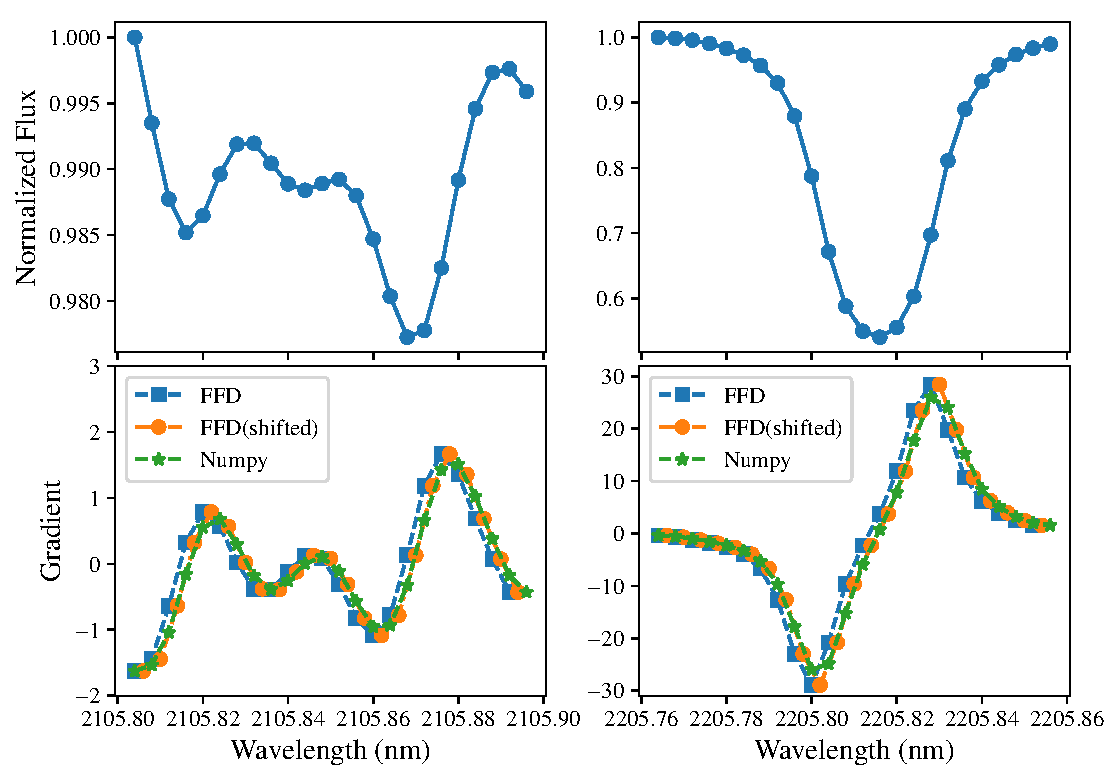
\includegraphics[width=0.85\linewidth]{figures/information-content/spectral_gradients}\\
    \caption[Comparing of numerical gradient alogithms.]{Visualization of the numerical gradient of some spectral lines.
        Top: The two spectral regions of a stellar spectrum: the left hand side contains short lines near the normalized continuum while on the right a single deep absorption line is shown.
        Bottom: The numerical gradients for the spectra shown in the top panels: the original {FFD} method is displayed with \emph{blue squares} while \numpy{} gradient is shown with \emph{green stars}.
        The \emph{orange circles} are the {FFD} version shifted to the mid-points between pixels for illustrative purposes.}
    \label{fig:gradients}
\end{figure}


%!TEX root = ../thesis.tex

\begin{table}
    \centering
    \caption[Affect of numerial gradient.]{The affect of the numerical gradient function on {RV} precision.
        The band label \(\rm VIS\) and \(\rm NIR\) indicate the full visible and \nir{} bands while  \(\rm CARM_{VIS}\)  and \(\rm CARM_{NIR}\) indicate the two wavelength bands of the {CARMENES} spectrograph.
        Column A is the RV precisions calculated using the {FFD} gradient.
        Column B contains the {FFD} gradient method but applied with a wavelength shift of \(\Delta\lambda/2\) in between pixels for this comparison only.
        Column C contains the RV precision calculation using the \npgradient{} function.
        The final two columns give the relative precision change between gradient method A and the other two, as a percentage.
        The {M0} spectra used here had no rotation, or instrument broadening performed and was normalized to a maximum of 1 in each band.
        The values given here are for accessing the relative precision change due to the different gradient methods only.}
    \begin{tabular}{ccccccc}
        \toprule
        %% Band & \(\lambda\) range\_min & wl\_max &  dy/dx   & gradient & Q(dy/dx) & Q(grad) & Q(frac) & {RV}(dy/dx) & {RV}\_adj &    {RV}(grad)    &    {RV}(frac\_grad)    & {RV}(frac\_adj)          \\
        Gradient method &  &  A &   B & C & (B-A)/A & (C-A)/A \\
        &   \(\lambda\) range & FFD & FFD+\(\Delta\lambda/2\) &  Numpy & \(\Delta\delta V\) ratio& \(\Delta\delta V\) ratio\\

        Band  & (\si{\micro\meter})  & \multicolumn{3}{c}{\(\delta V_{rms}\) (\mps{})}  & (\%) & (\%) \\
        \midrule
        VIS & 0.38 -- 0.78 & 16.1 & 16.2 & 16.9  & 0.6 & 4.9\\
        \(\rm CARM_{VIS}\) & 0.52 --  0.96 & 20.9 & 21.0 & 22.0 & 0.3 & 5.2 \\
        Z & 0.83 -- 0.93 & 76.9 & 77.0 & 78.8  & 0.1 & 2.5\\
        Y & 1.00 -- 1.10 & 78.3 & 78.5 & 83.8 & 0.2 & 7.0 \\
        J & 1.17 -- 1.33 & 149.3 & 149.4 & 156.4 & 0.1 & 4.7 \\
        H & 1.50 -- 1.75 & 119.4 & 119.5 & 122.3 & 0.1 & 2.5 \\
        K & 2.07 -- 2.35 & 153.4 & 153.7 & 157.7  & 0.2 & 2.8\\
        \(\rm CARM_{NIR}\) & 0.96 -- 1.71 & 46.1 & 46.2 & 48.0 & 0.1 & 4.2 \\
        NIR & 0.83 -- 2.35 & 36.9 & 36.9 & 38.2 & 0.1 & 3.6  \\
        \bottomrule
    \end{tabular}\label{tab:numerical_gradients}
\end{table}


\cref{fig:gradients} visualizes two small spectral regions with the gradients computed with the original {FFD} and the \npgradient{} methods.
The top panels contain a small section of a simulated spectrum, comprised of three small blended lines, and a large single line respectively.
The derivative of the spectrum for the {FFD} method (blue squares) and \npgradient{} method (green stars) are shown in the bottom panels.
The \emph{orange circles} are the same as the {FFD} method but shifted horizontally to the midpoints between the pixels for which the gradient is calculated at.
This is for illustrative purposes and to assess the effect of this offset when calculating the pixel weights.

There are three notable features observed between gradient methods.
The first, which is expected from the {FFD} formulation is that the {FFD} gradient is offset to the left by half of a pixel.
The second is that when the horizontal offset is adjusted (orange circles) the two gradients lie along the same curve.
Both methods are trying to approximate the real gradient function of the spectrum so it is expected that they should agree.
The most important feature observed in this though is that there is a slight over-estimate of the gradient by the {FFD} method at the peak of each extrema.
The points of highest gradient are always from the {FFD} method (blue/orange).
This is the case for all spectral lines and as the optimal pixel weights are proportional to the gradient squared the {FFD} method will apply slightly higher pixel weights to these values, two points per line in the spectrum.
Therefore, the {FFD} gradient produces a slightly smaller \(\delta V_{\rms}\) error compared to the more precise gradient function.

The numerical differences between the gradient methods on the relative {RV} precisions is given in \cref{tab:numerical_gradients}.
The \(\delta V_{\rms}\) is calculated using both gradient methods on a {PHOENIX-ACES} spectrum with \Teff{}=3900\K{}, corresponding to {{M0}} spectral type.
The full theoretical precision is calculated (no telluric masking applied) with no rotational or instrumental broadening and with the maximum of the continuum of each band scaled to 1.
In this case the {RV} precisions are not comparable between bands and are used only to assess the direct effect of the numerical gradient.
The band names and the spanned wavelengths are given along with the {RV} precision calculated with different gradients in columns A, B, and C.
A is the original {FFD} method, B is the {FFD} method offset by \(\Delta\lambda\), and C is the \npgradient{}.
The \(\delta V\) ratios are the relative difference in {RV} when changing from method A (the original {FFD}) to methods B and C.

As the pixel weights from \cref{eqn:optimal_weight} are proportional to \({\lambda}^{2}\), column B was computed to assess the affect of the slight wavelength offset on the {RV} precision, visible in \cref{fig:gradients}.
\cref{tab:numerical_gradients} shows that wavelength offset of \(\Delta\lambda/2\) contributes 0.1--0.6\% to the {RV} precision values, an order of magnitude smaller than the change from A to C.
Changing from the {FFD} method to \npgradient{} to use the gradient from \numpy{}, increases the \(\delta V_{\rms}\) by 2.5--7\%, decreasing the {RV} precision.
After ruling out the wavelength offset with B, it is assumed that this difference is due mainly to the over-estimated gradient from the {FFD} method, shown in \cref{fig:gradients}

Changing the method of numerical derivatives will change all the precision values given in~\citet{figueira_radial_2016}.
This has a small impact on the precision compared to other components of the {RV} precision.
For instance from \cref{eqn:snr_relation} an increase in \(\delta V_{\rms}\) of between 2.5--7\% could equally be caused by a small decrease in the \snr{} from 100 (the value used in~\citet{figueira_radial_2016}) to between 95--98.

The current version of the software is now implemented with the gradient method provided by the \numpy{} package, and as such there is a small difference in {RV} precision values calculated, compared to~\citet{figueira_radial_2016}.

\subsection{Masking Function}
\label{subsec:masking_function}
Another change made to the software is in the application of the masking function, and the treatment of telluric lines.
As suggested in~\citet{connes_absolute_1985} and~\citet{bouchy_fundamental_2001} a custom masking function can be applied to the individual pixel weights in \cref{eqn:optimal_weight}, such as:
\begin{equation}
W'(i) = W(i)\mathcal{M}(i),\label{eqn:mask_function}
\end{equation}
where \(\mathcal{M}(i)\) is the masking function and \(W'(i)\) are the modified pixel weights.
This masking function can be used in particular for the removal of telluric lines, setting those weights to zero and is in essence what is done when wavelength selection is performed: zero weight is assigned to all pixels outside the desired wavelength range.

This masking function can be used to easily apply the three conditions presented in~\citet{figueira_radial_2016}.
The three masking functions incorporated into \eniric{} are defined here, followed by the quantification of how they differ from the previous implementation.
The subscripts on the masking functions \(\mathcal{M}\) correspond to the three conditions.
\begin{align}
{\mathcal{M}}_{1}(i) &= 1 \label{eqn:mask1}\\
{\mathcal{M}}_{2}(i) &= \begin{cases}
0, \hspace{1em} T(i) < \tau\\
1, \hspace{1em} T(i) \ge \tau\\
\end{cases}\label{eqn:mask2}\\
{\mathcal{M}}_{3}(i) &= {T(i)}^{2} \label{eqn:mask3}
\end{align}

Here, \(T(i)\) is the telluric transmission spectrum, while \(\tau\) is the transmission depth cut-off.
For instance to mask out telluric lines deeper than 2\% the value of \(\tau\) would be set at 0.98.

\begin{itemize}
    \setlength\itemsep{-0.2em} % Remove spacing on list.
    \item Condition~\#1:
    The first mask, \({\mathcal{M}}_{1}\), is the simplest case in which all pixel weights are treated equally.
    No telluric line masking is considered, and the full theoretical precision of the spectrum is obtained.
    
    \item Condition~\#2:
    In the second mask, \({\mathcal{M}}_{2}\), the telluric line transmission, \(T(i)\) is used to create a boolean mask of 0's and 1's.
    When applying this mask to the pixel weights, the pixels that are affected by telluric lines are given a weight of 0, removing their contribution to \(\delta {V}_{\rms}\).
    Accounting for seasonal variation in Earth's barycentric motion can be easily incorporated into this mask by increasing the width of the regions masked out.
    
    \item Condition~\#3:
    This condition assumes the application of perfect telluric correction in which variance (photon noise contribution) in the denominator of \cref{eqn:optimal_weight} is amplified by the telluric correction.
    In~\citet{figueira_radial_2016} the pixel weighting for this condition becomes:
    \begin{equation}
    W(i) = \frac{{\lambda}^{2}(i) {({\partial {A}_{0}(i)}/{\partial \lambda(i)})}^{2}}{A_0(i) + {\sigma}^{2}_{D}/{T(i)}^{2}} \label{eqn:optimal_weight_transmission}
    \end{equation}
    As the telluric transmission spectrum is a division in the denominator it is equivalent to multiplying the pixel weights by a mask of the form \({\mathcal{M}}_{3}\).
\end{itemize}

Having the three masks defined in this way makes the implementation of the pixel weight calculations simpler.
In the original version there were three separate implementations, one for each condition.
With three separate functions there is more room for mistakes, which there was with Condition~\#2 as will be discussed in \cref{subsec:condition_two_bug}.
In the new implementation there is a single function that calculates the pixel weights from the spectrum, which can incorporate a masking function.
The three masks mentioned here are implemented and used, and there is even the option for a user defined pixel mask to be used.


\subsubsection{Masking order}
\label{subsubsec:masking_order}
The order in which the masking is performed was found to affect the recovered {RV} precisions.
That is, the application of weight masking must be applied to the spectrum only after the calculation of the pixel weights.

In the original implementation of Condition~\#2, the full spectral band was split into small wavelength regions (sub-spectra) in between the telluric lines, following the masking by \(\mathcal{M}_{2}\).
The \(\delta V_{\rms}\) was calculated using the {FFD} gradient for each small region with the results combined as the error on the weighted average in \cref{eqn:weighted_average_error}.
Analytically this result is identical to masking out the pixel weights with \({\mathcal{M}}_{2}\) but, in practice, it is not when numerically implemented.

When the spectrum is split into many small sections the number of edges increases and so does the number of pixels affected by edge effects.
As shown in \cref{sec:numerical_gradient} the {FFD} method only computes \(n-1\) gradients from \(n\) pixels: the last pixel is removed/lost.
A spectrum split into \(m\) sub-spectra will therefore lose \(m\) pixels due to this edge effect.
This is in contrast to computing the weights first and then masking or splitting the spectrum in which only 1 pixel from the full spectrum is lost with the {FFD} gradient.
Even the \npgradient{} is not immune to the edge effects in the sub-spectra when the spectral splitting is performed first.
Although there are no pixels lost, the first and last pixels of each sub-spectra are computed using forward or backward differences, rather than central differences (as they would be in the full spectrum).
Hence, the gradients obtained and subsequent pixels weights of the sub-spectra edge pixels are slightly altered due to the spectral splitting occurring first.

The effect of masking and splitting the spectrum before and after calculating the pixel weights is quantified in \cref{tab:mask_ordering}.
The columns labelled \emph{Split} represents splitting the spectrum before calculating the pixel weights, while the columns labelled \emph{Mask} calculate all the pixel weights first and then apply the \({\mathcal{M}}_{2}\) mask.
The difference in {RV} precision between both situations and for both gradient methods are provided.
For the {FFD} gradient, changing the ordering of splitting/masking from before the weight calculation to after decreases (improves) the {\(\delta V_{\rms}\)} by 0.2--0.7\%, while for \npgradient{} the \(\delta V_{\rms}\) is increased but at an order of magnitude smaller than the {FFD} method, only between 0.01--0.13\%.
In this case the {FFD} method has a larger change observed due to the addition of the \(n-2\) pixels that were originally lost.
With the \npgradient{} all pixels are always included, and the end values only slightly change.
The last column of \cref{tab:mask_ordering} is the difference ratio between the \emph{Mask} column of both gradient methods.
These are consistent with the values obtained in \cref{tab:numerical_gradients} with the differences between the two gradient methods of 2--7\%.
This table also shows that the difference induced on the {RV} precisions from changing the order of weight calculation and masking is 1--2 orders of magnitude smaller than the change from the new gradient method.

\Eniric{} has been adjusted to consistently apply the masking after the pixel weights are calculated, simplifying the implementation.
This retains the most pixels, with the most accurate pixel weights (less edge effects).
It has also been changed to only apply the \({\mathcal{M}}_{2}\) and not split the spectrum into small sub-spectra then perform the weighted error calculation of \cref{eqn:weighted_average_error}.
The functionality to perform the weighted error is still present and can be used to combine the {RV} precision of larger spectral chunks, such as the separate \nir{} bands or the different spectral orders in a cross-dispersed spectrograph.

%!TEX root = ../thesis.tex

\begin{table}
    \centering
    \caption[{RV} precision with different splitting.]{Relative {RV} precision difference for Condition~\#2 due to spectral splitting and order of applying the pixel mask.
        The input parameters were for an {M0} spectral type spectrum, with $\vsini=1.0$ and R=100\,000.
        The \(\Delta\)ratios are the percentage difference between \textit{Split} and \textit{Masked} implementations while using the same gradient method.
        The last column is the ratio between the \textit{Masked} implementations using the {FFD} and \npgradient{} methods and are consistent with \cref{tab:numerical_gradients}.
        }
    \begin{tabular}{c|ccc|ccc|c}
        \toprule
        & Split & Masked & \(\Delta\)Ratio & Split & Masked & \(\Delta\)Ratio & Masked \\
        Gradient & \multicolumn{3}{c|}{FFD} & \multicolumn{3}{c|}{Numpy} & \(\Delta\)Ratio\\
        Band & \mps{} & \mps{} &  \%  & \mps{} & \mps{} &   \% & \% \\
        \midrule
        Z &  7.42 &  7.38 & -0.66 &  7.76 &  7.77 & 0.13 & 5.3\\
        Y &  4.75 &  4.74 & -0.22 &  5.06 &  5.06 & 0.06 & 6.8\\
        J & 18.58 & 18.53 & -0.29 & 19.57 & 19.57 & 0.01 & 5.6\\
        H &  6.08 &  6.05 & -0.53 &  6.25 &  6.26 & 0.08 & 3.5\\
        K & 32.21 & 32.14 & -0.22 & 33.48 & 33.49 & 0.05 & 4.2\\
        \bottomrule
    \end{tabular}\label{tab:mask_ordering}
\end{table}


The ordering of the masking does not affect the results of Condition \#1 or \#3 that were not split into sub-spectra to calculate the {RV} precisions.
Although there are differences from the old and new implementation of Condition \#2 (splitting to only masking) the differences observed between~\citet{figueira_radial_2016} and this work are dominated by a found bug, see \cref{subsec:condition_two_bug}.


\subsection{\snr{} scaling}
\label{subsec:snr_scaling}
For the analysis of relative synthetic spectral precision between different spectra, a common reference point is needed.
Similarly to~\citet{figueira_radial_2016} in \cref{subsec:orginal_snr_scaling} this is achieved by normalizing the synthetic spectra to a specific \snr{} per resolution element level at a particular wavelength.
However, unlike~\citet{figueira_radial_2016}, this is not held fixed at \snr{}=100 in the middle of the \emph{J}-band at 1.25\um{}.

\Eniric{} now contains an automated \snr{} scaling procedure (\cref{eqn:snr-scaling-factor}), to remove the need for the hard-coded scaling values, and extends the precision calculations to any \snr{}, sampling, and wavelength specifications.

The procedure first identifies the wavelength value \(\lambda^\prime\) to perform the scaling at; this can be either a user defined wavelength value, or more commonly the centre of a user selected band is automatically computed from the configured band limits.
The number of pixels within one resolution element \(\lambda/R\), is defined by the sampling, \(\mathrm{s}\), used to interpolate the spectrum \cref{subsec:orginal_interpolation}.
The photons within one resolution element are calculated by summing \(\mathrm{s}\) pixels, (\(N=\sum\limits^{\mathrm{s}}{{A}_{0}}\)), centred on \(\lambda^\prime\).
The current \snr{} of the resolution element is calculated as \(\snr{} = \sqrt{N}\) assuming a large N.
A scaling factor, \(SF\), is defined so that when it is multiplied by the spectrum, the \snr{} of the resolution element at \(\lambda^\prime\) becomes the desired value, \({\snr{}}_{\textrm{desired}}\):
\begin{equation}
SF =  \frac{\sqrt{\sum\limits^{\mathrm{s}} A}} {\snr{}_{desired}}. \label{eqn:snr-scaling-factor}
\end{equation}

Automating the calculation of the scaling factor enabled several new scenarios to analyse the relative precisions, not previously possible.
Four are given here:
\begin{itemize}
    \setlength\itemsep{-0.3em} % Remove spacing on list.
    \item The ability to easily analyse new spectral models, not just the four spectra corresponding to {M0}, {M3}, {M6}, {M9} spectral types, which scaling factors had been manually calculated for.
    \item The ability to scale to a \snr{} per pixel value other than 100.
    \item Allow for the correct scaling when a different sampling, \(\mathrm{s}\), is used.
    Not just restricted to \(\mathrm{s}\)=3.
    \item Allow for relative precisions to be referenced to a different band or wavelength.
    Results are not limited to being referenced relative to the \textit{J}-band.
\end{itemize}

This last point is of note as it allows the relative precisions not to be tied to a single band, allowing the testing of different \snr{} values achievable at different wavelengths.
For instance, all {RV} precisions can now be calculated relative to a given \snr{} at the centre of the \textit{K}-band.
This was important for computing~\citet{figueira_radial_2016}-like precisions requested for the {NIRPS} and {SPIRou} Exposure Time Calculators ({ETC}).
{NIRPS} specifically requested precision values at a \snr{} relative to the individual bands (the precision of the \emph{K}-band spectrum relative to \snr{}=100 at the centre of the \emph{K}-band), while {SPIRou} requested precisions relative to the \emph{J}- and \emph{H}-bands only.
These calculations were not easily possible in the original code version, and this extension has made computations for different \snr{} level and reference points easy to calculate, with minimal configuration.

The default values set in \eniric{} match the~\citet{figueira_radial_2016} value, a \(\mathrm{s}\)=3 and \snr{}=100 in the \emph{J}-band.
The centre of each band was visually checked to ensure that default, central band reference locations did not coincide with a spectral line.
If the reference point was automatically chosen at the centre of an absorption line, then the counts \(N\) would be lower and the spectrum would be scaled to a higher continuum.
This would artificially decrease (improve) the \(\delta V_{\rms}\) recovered.
At rest, the centres of the \emph{Z}-, \emph{Y}-, \emph{J}-, \emph{H}-, and \emph{K}-bands as defined in \cref{tab:infrared_bands} do not coincide with a spectral line. However, if any Doppler shifting is performed to move the spectral lines, then care must be taken to ensure the correct scaling is applied to the continuum.

As shown in \cref{eqn:snr_relation} the {RV} precision is inversely proportional to the \snr{} level.
To access the relative {RV} precision of any of the values calculated at a different \snr{} level you can apply the following:
\begin{equation}
{\delta V}_{{\snr{}}_{2}} = {\delta V}_{{\snr{}}_{1}} * \frac{{\snr{}}_{1}}{{\snr{}}_{2}},
\end{equation}
where \(\delta {V}_{{\snr{}}_{1}}\) is the relative precision calculated at \({\snr{}}_{1}\) and \({\delta V}_{{\snr{}}_{2}}\) is the new precision if observed instead with a \snr{} of \({\snr{}}_{2}\).


\subsection{Atmospheric masking bug}
\label{subsec:condition_two_bug}
Applying testing practises of \cref{subsec:automated_testing} during the extension of \eniric{} revealed an error in the application of Condition~\#2 in~\citet{figueira_radial_2016}.
When the telluric line mask was broadened to account for the barycentric motion of the Earth, and a requirement requiring three consecutive pixels (the sampling rate) to exceed the cut-off limit to be considered masked out, there was a software bug.
This meant that the masking applied for Condition \#2 was incorrect and not physically meaningful.
It essentially randomly masked portions of the spectra, not physically meaning full to the treatment of the telluric lines.
The synthetic spectra did not have telluric line contamination themselves, but the proportion and location spectrum supposed to be mask to represent telluric contamination masking applied was incorrect.

A check for this issue was discovered using this unit test (\cref{lst:masking_unit_test}), written under the \href{https://docs.pytest.org}{pytest} framework.
Essentially, this takes a given transmission (telluric line) spectrum and creates a telluric mask at a line depth of 2\%.
It then transforms the mask by the function \pythoninline{barycentre_broaden()}, the function under test here, which performs the \(\pm30\)\kmps{} barycentre broadening to account for the yearly motion of the Earth, and consecutive pixel check.
The assert statement performs the actual test, checking that if the new broadened mask is applied to the original transmission spectrum, then all values are greater or equal to the masking limit.
That is, the telluric lines are still completely masked out.

This is not the only test required to sufficiently test the ``correctness'' of \pythoninline{barycentre\_broaden()}, but it is a simple unit test\footnote{A unit test only tests single specific piece of code or functionality at a time.} that would have caught the bug that was present.
%\begin{lstlisting}[language={python}, caption={Example unit test to catch the masking bug.\ The assert statement checks that the mask continues to remove all telluric lines deeper than 2\%.}, label={lst:masking_unit_test}]
%def test_telluric_masking(wavelength, transmission):
%    """Check the mask still masks out all telluric lines > 0.98 after
%    broadening the mask to account for the barycentre motion."""
%    mask = telluric_mask(transmission, depth=0.98)  # Create mask
%    mask = barycentre_broaden(wavelength, mask)     # Extend mask
%    assert numpy.all(transmission[mask] >= 0.98)    # Assert condition
%\end{lstlisting}
\begin{python}[caption={Example unit test to catch the masking bug.\ The assert statement checks that the mask continues to remove all telluric lines deeper than 2\%.}, label={lst:masking_unit_test}]
def test_telluric_masking(wavelength, transmission):
    """Check the mask still masks out all telluric lines > 0.98 after
    broadening the mask to account for the barycentre motion."""
    mask = telluric_mask(transmission, depth=0.98)  # Create mask
    mask = barycentre_broaden(wavelength, mask)     # Extend mask
    assert numpy.all(transmission[mask] >= 0.98)    # Assert condition
\end{python}
Due to this bug the published {RV} precision values for Condition~\#2 in~\citet{figueira_radial_2016} are all incorrect.
As the masking was unevenly applied the new ``correct'' {RV} precision values do not all change in the same direction or in the same proportion.
For example, the largest difference is seen in the \emph{J}- and \emph{K}-bands, with changes over 20\mps{}, while other wavelength bands are essentially unchanged.
The differences can be seen in the shaded areas of \cref{fig:figueria_comparision} comparing the~\citet{figueira_radial_2016} results to the updated values, with the upper edge defined by Condition \#2.
Even though there is an error with the values of Condition~\#2 they do not change the overall conclusions of the paper.



%!TEX root = ../../thesis.tex

\section{RV precision update}
\label{sec:rv_precision_values}

\begin{figure}
    \centering
    \begin{tabular}{cc}
        \multicolumn{2}{c}{\citet{figueira_radial_2016}}\\
        \multicolumn{2}{c}{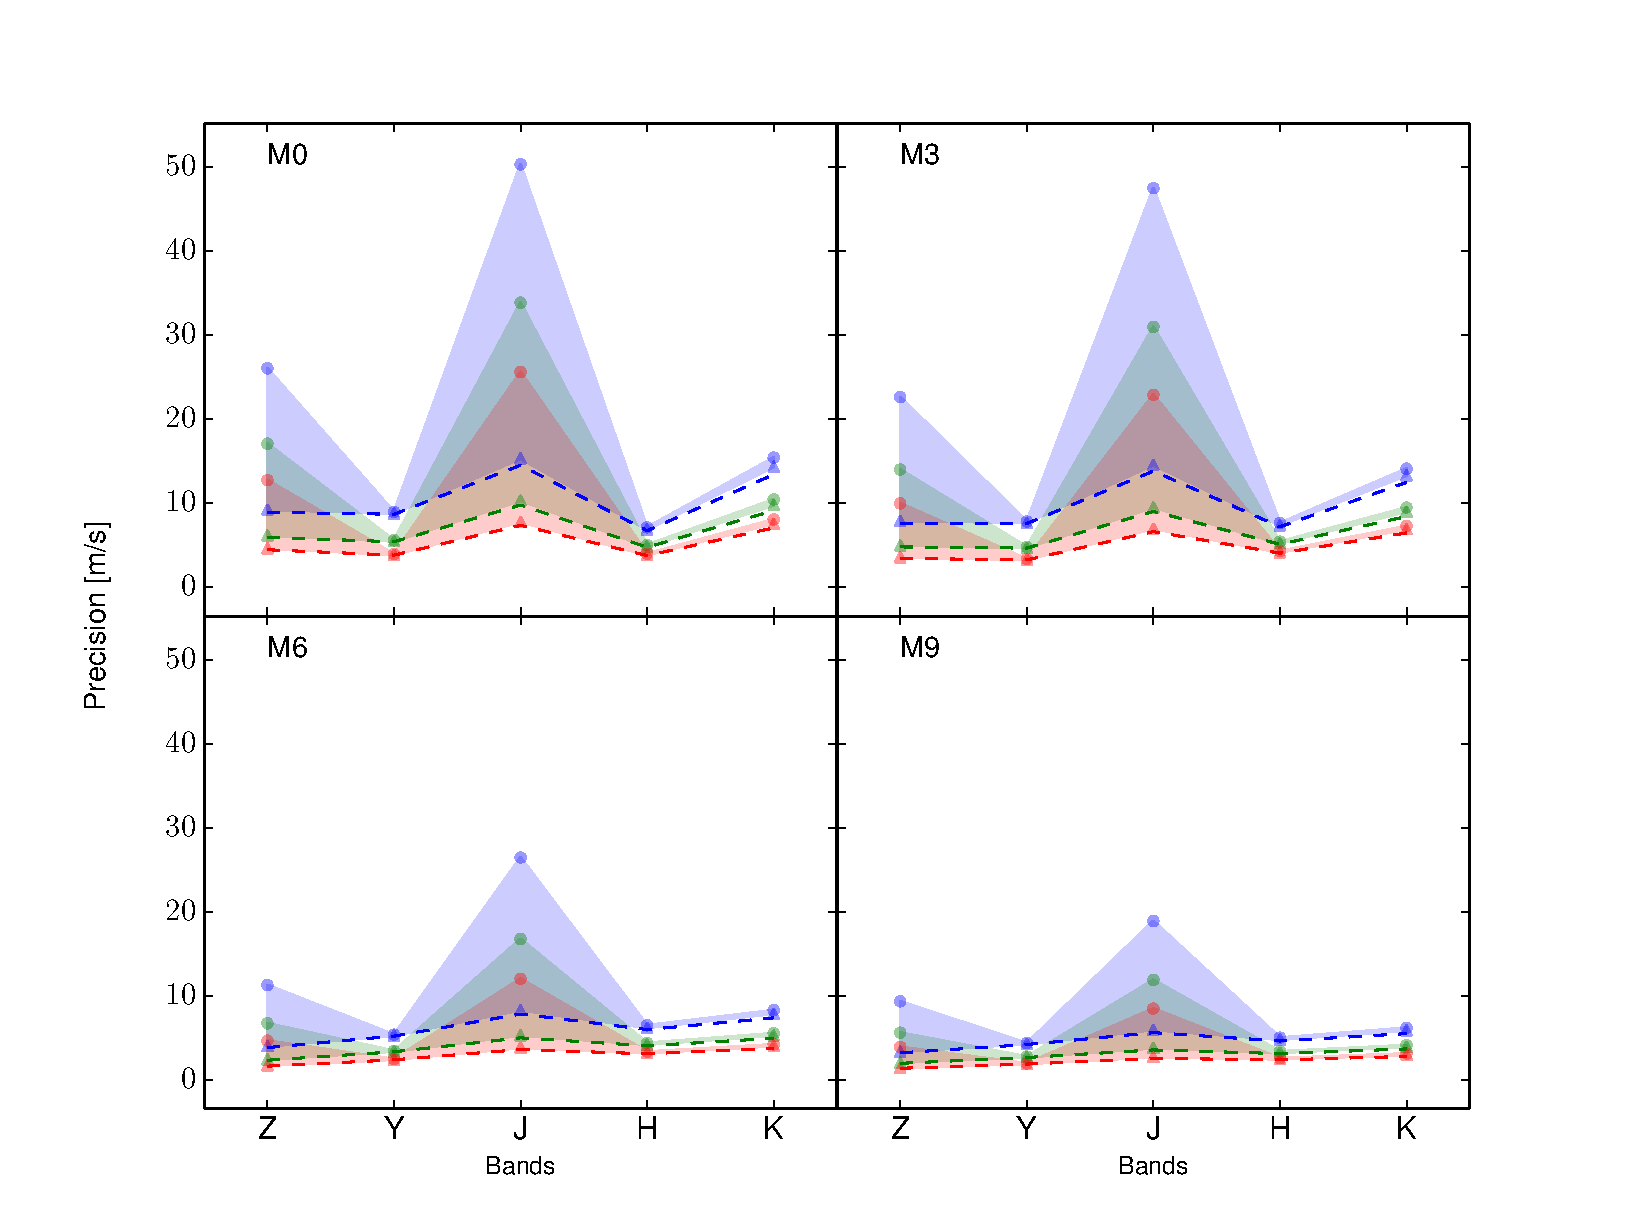
\includegraphics[width=0.48\linewidth]{figures/information-content/Rvprec_vsini1.pdf}}\\
        {PHOENIX-ACES} & {BT-Settl}\\
        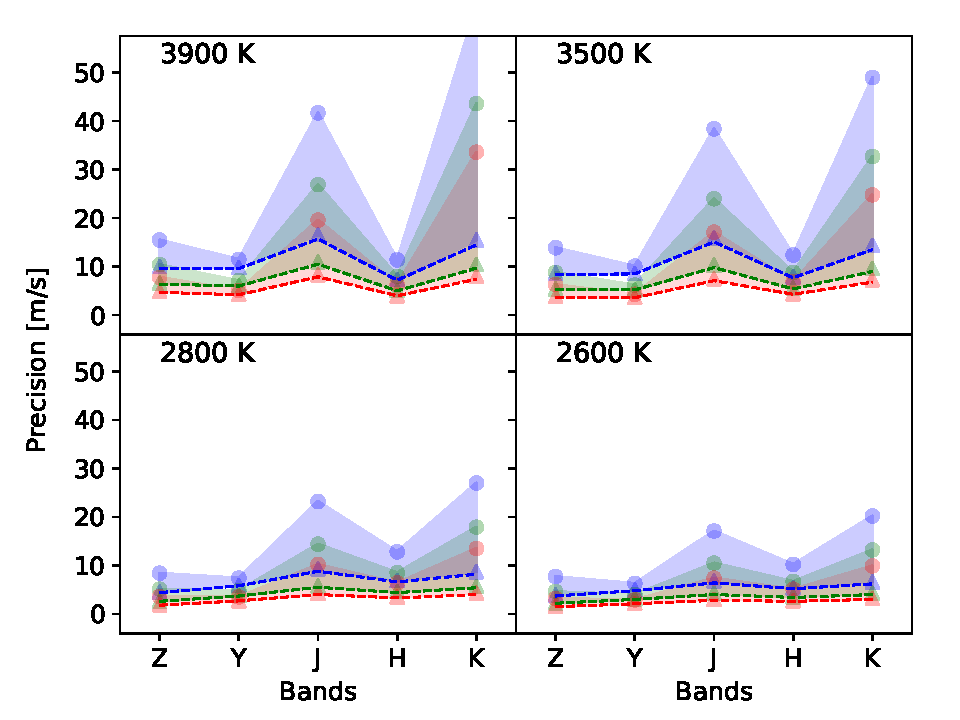
\includegraphics[width=0.47\linewidth]{figures/information-content/aces_4panel} &
        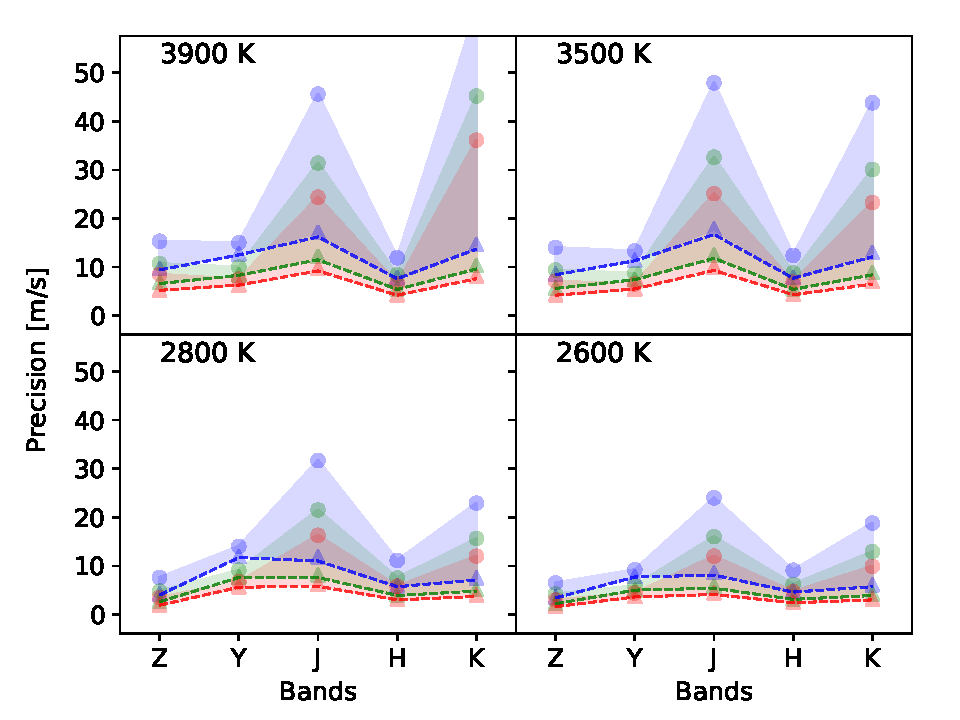
\includegraphics[width=0.47\linewidth]{figures/information-content/btsettl_4panel} \\
    \end{tabular}
    \caption[Comparision of {RV} precision results to~\citet{figueira_radial_2016}.]{Comparison of the updated precision values to the original values.
        Top: Figure~1 from~\citet{figueira_radial_2016}.
        Bottom: Updated precision values computed using \eniric{} using the {PHOENIX-ACES} (left) and the {BT-Settl} (right) models.
        Each panel shows the precision achieved as a function of spectral band for stars with a rotational velocity of \Vsini=1.0\kmps{} and spectral types {M0}~(3900\K), {M3}~(3500\K), {M6}~(2800\K), and {M9}~(2600\K{}).
        The dashed line represents the theoretical limits imposed by Condition~\#1, and the filled area represents the values within the limits set by Conditions~\#2 (circles) and \#3 (triangles); blue, green, and red represent the results obtained for resolutions of 60\,000, 80\,000, and 100\,000, respectively.
        The spectra were normalized to have a \snr{} of 100 per resolution element as measured at the centre of the \emph{J}-band.}
    \label{fig:figueria_comparision}
\end{figure}

As detailed in the \cref{sec:eniric} updating the software introduced several changes that affect the {RV} precisions values slightly, the numerical gradient, and the masking order for Condition~\#2 and more importantly the bug also found with Condition~\#2.

The 180 spectral combinations from \citet{figueira_radial_2016}, are repeated here using \eniric{} to have an updated and corrected table of relative {RV} precisions.
This table is given in \cref{tab:rv_aces_btsettl}, calculated using the {PHOENIX-ACES} spectra and also the {BT-Settl} models.
 
The precision changes are visually represented in \cref{fig:figueria_comparision} by comparing Figure~1 of \citet{figueira_radial_2016} (top) to the updated precisions using \eniric{} with the {PHOENIX-ACES} (bottom-left) and {BT-Settl} (bottom-right) models.
Each panel shows the precision achieved as a function of spectral band for stars with a rotational velocity of \Vsini=1.0\kmps{} and spectral types {M0}~(3900\K), {M3}~(3500\K), {M6}~(2800\K), and {M9}~(2600\K).
The dashed line represents the theoretical limits imposed by Condition~\#1, and the filled area represents the values within the limits set by Conditions~\#2 (circles) and \#3 (triangles); blue, green, and red represent the results obtained for resolutions of 60\,000, 80\,000, and 100\,000, respectively.
The spectra were normalized to have a \snr{} of 100 per resolution element as measured at the centre of the \emph{J}-band.

The values for Condition~\#1 and \#3 only have small differences which is barely noticeable, while Condition~\#2 has large band dependant changes, shown by the change in the shaded areas.
For example note that \emph{Z} and \emph{J}-band {RV} precisions decrease with the new results, while the \emph{K}-band gets substantially worse.
This occurs because the software did not mask many of the regions affected by telluric lines, where as in the new results, a significant portion is masked out due to the overlap of telluric lines, leading to a higher \(\delta V_{\rms}\) value.
The \emph{H}-band also sees a small increase in \(\delta V_{\rms}\).

As stated previously the discovery of the bug affecting telluric masking does not change the conclusions of \citet{figueira_radial_2016}.
These updated {PHOENIX-ACES} values will be published in an upcoming work as an amendment to the \citet{figueira_radial_2016} values.

In comparing the bottom two panels between the {PHOENIX-ACES} and {BT-Settl} models, there are only small differences, most identifiable in the Condition~\#2 values of the \emph{J}-band.
This shows again that the {PHOENIX-ACES} and {BT-Settl} models are fairly consistent.
This was also visually observed in \cref{subsec:phoenix_comparision}.


\section{Metallicity and \texorpdfstring{\Logg{}}{Logg}}
\label{sec:metallicity_logg}
\begin{figure}
    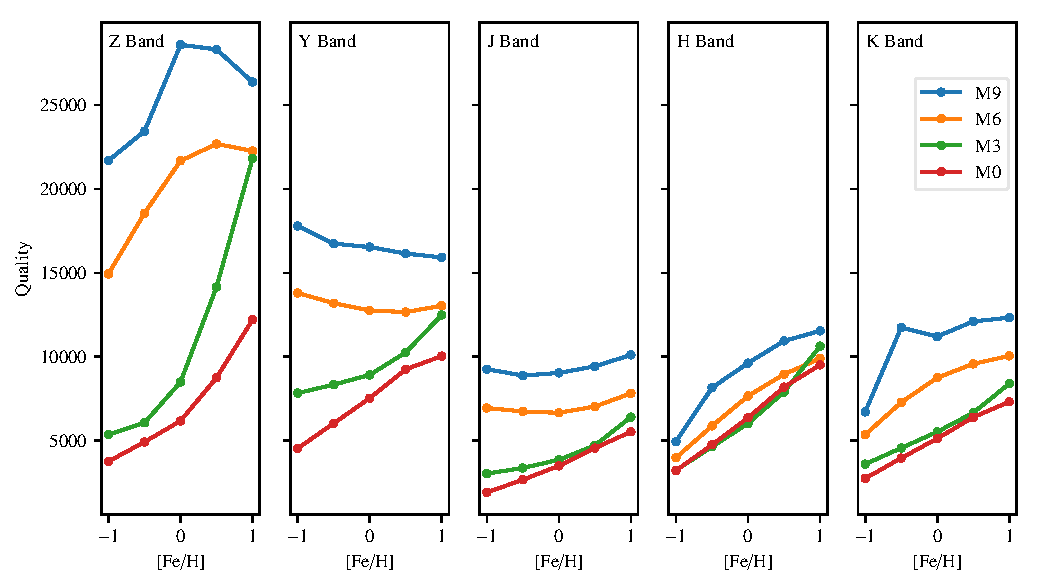
\includegraphics[width=0.95\linewidth]{figures/information-content/metalicity_effect.pdf}\\
    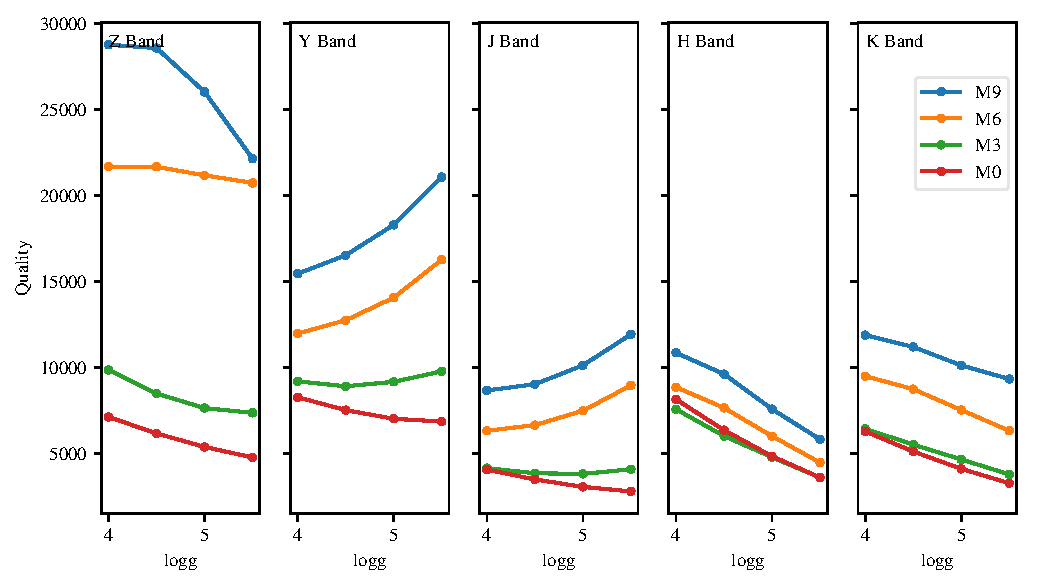
\includegraphics[width=0.95\linewidth]{figures/information-content/logg_effect.pdf}
    \caption[Quality factor verse \feh{} and \Logg{} for different spectral types and wavelength bands.]{Quality factor changes across spectral type and bands for variations in \feh{} and \Logg{}.
        Broadening values are R=100\,000 and \Vsini{}=1.0\kmps{}.
        Top: Quality factor variation of \feh{} between -1.0 to 1.0 at a fixed \Logg{}=4.5.
        Bottom: Quality factor variation of \Logg{} between 4 and 5.5 with fixed \feh{}=0.0.
        Note a higher quality factor corresponds to an increased {RV} precision.}
    \label{fig:logg_metalicity_deviations}
\end{figure}

With the ability to explore a wider range of parameters the range of {PHOENIX-ACES} models were extended to explore the affect of \Logg{} and \feh{} on the relative {RV} precision.
Remember that \Logg{} is a measure of the stellar surface gravity, the gravitational acceleration at the equator expressed in {cgs} units of \si{\centi\metre\per\second\squared} then taking the logarithm of base-10.
The surface gravity is \(g \propto \frac{M}{R^{2}}\) so larger \Logg{} values correspond to stars with smaller radii.
While the metallicity, \feh{}, is a measure of the abundance of elements heavier than Hydrogen and Helium, it is often measured as the ratio of Iron to Hydrogen relative to the Sun.
That is a \feh{}=0 has the same metal ratio as the Sun, a positive \feh{} has more metals, and a negative \feh{} has less metals than the Sun.
The higher abundance of metals creates stronger absorption lines.

\Eniric{} was used to compute the spectral quality factor, \(Q\) (\cref{eqn:quality_factor}), and {RV} precision for all {PHOENIX-ACES} models with \Logg{} between 4.0--5.5 and \feh{} between -1--1, inclusive.
The spectral factor is used for the comparison following \citet{artigau_optical_2018} in which it was used to compare between models, and observed spectra, independent of the flux levels.
Since \(Q\) is inversely proportional to \(\delta V_{\rms}\) a higher \(Q\) is better.

The spectral quality factor variations for the {M-dwarf}s {M0}, {M3}, {M6}, {M9}, with a broadening of R=100\,000 and $\vsini=1.0$\kmps{} across the \nir{} bands is shown in \cref{fig:logg_metalicity_deviations}.
The top row shows the quality for model spectra with a fixed \Logg=4.5 but having a variable \feh{} between -1.0 to 1.0.
The bottom row shows the opposite: a fixed \feh{}=0.0 while the \Logg{} is varied between 4 and 5.5.
The five separate plots in each row represent the \nir{} wavelength bands \emph{Z}--\emph{K} and the four different coloured lines are the different M-dwarfs (blue {M9}, orange {M6}, green {M3}, red {M0}).

Multiple effects are observed in this figure which are identified below, organized into the separate bands.
Note that the cooler M-dwarfs (M6, {M9}) almost consistently have higher spectral quality factors, corresponding to lower \({\delta V_\rms{}}\) (improved relative precision), if observed at the same relative \snr{} level, as can be seen in \cref{fig:figueria_comparision}.

\begin{itemize}
\item  \emph{Z}-band\\
The \emph{Z}-band has a large separation in spectral quality due to spectral type, this is because the continuum of the \emph{Z}-band is severely eroded in the spectra of late M's as they cool.
Each spectral type also behaves very differently to a change in \feh{} and \Logg{}.
For {M0} and {M3} there is a small increase with increasing \feh{} below solar metallicity; above solar metallicity the slopes of the lines dramatically increase, especially for {M3} where the quality more than doubles between a \feh{} value of 0.0 to 1.0.
For {M6} and {M9} there is a sharp decrease in quality as \feh{} falls below solar metallicity (0.0).
The quality seems to peak between \feh{}=0.0--0.5 and begins to decrease at higher metallicity.

As \Logg{} increases in the \emph{Z}-band there is a decrease in spectral quality.
There is a consistent and large separation between early and late M's that.
The quality for {M6} is very shallow, while for {M9} the quality is nearly flat for \Logg{}=4.0 and 4.5 but then decreases sharply at higher \Logg{}.

\item \emph{Y}-band and \emph{J}-band \\
The spectral quality in the \emph{Y}-band is interesting, as the quality appears to converge and diverge with increasing \feh{} and \Logg{} respectively.
For {M0} and {M3} there is an increase in quality as the metallicity increases in both bands, while for {M6} and {M9} there is a decrease in quality in the \emph{Y}-band, converging together beyond \feh{}=1.0.
In the \emph{J}-band the {M6} and {M9} are almost flat with a gentle decrease then increase in quality.

For the \Logg{} variation the opposite occurs.
As the \Logg{} increases from 4.0 to 5.5 {M0} has a small gradual decrease in the spectral quality with {M3} remaining relatively flat.
{M6} and {M9} both increase with increasing \Logg{} so overall there is a divergence in the spectral quality at a larger \Logg{} in both bands.

\item \emph{H}-band and \emph{K}-band \\
The \emph{H}-band and \emph{K}-band also have similar patterns between \feh{}, \Logg{} and quality for all spectral types, with only a small change between the different spectral types.
The spectral quality increases fairly consistently as \feh{} increases and decreases with an increase in \Logg{}.
There does however, appear to be one point that looks out of place in the {M9} spectrum with \feh{}=-0.5.

\end{itemize}

Looking at the bigger picture, there is a striking difference in the quality between the bands.
For the {M0} and {M3} spectra the quality mostly stays under 10\,000, apart from a four points in the \emph{Z} and \emph{Y}-bands at high \feh{}.
For the cooler {M6} and {M9} quality values however there is a large contrast between the \emph{Z} and \emph{Y}-bands, which have a much higher quality, and the other three bands which have a similar quality level.

This difference in spectral quality in the \emph{Z}-band becomes apparent when visualizing the spectra.
The \emph{Z}-band and \emph{J}-band spectra for all four spectral types from \citet{figueira_radial_2016} are reproduced here in \cref{fig:z_and_j_spectra}.
They show flux as a function of wavelength in the \emph{Z}-band (top) and \emph{J}-band (bottom) for a \Vsini{}=1.0\kmps{} and spectral types {M0}, {M3}, {M6}, and {M9} (\textit{top} to \textit{bottom} panels), when seen at a resolution of 100\,000.
The \emph{Z}-band has substantial erosion of the continuum in the {M6} and {M9} spectra, compared to the other spectra, even of the same spectral type.
The higher number of lines in the M8 and {M9} spectra show why the spectral quality is higher.

\begin{figure}
    \centering
    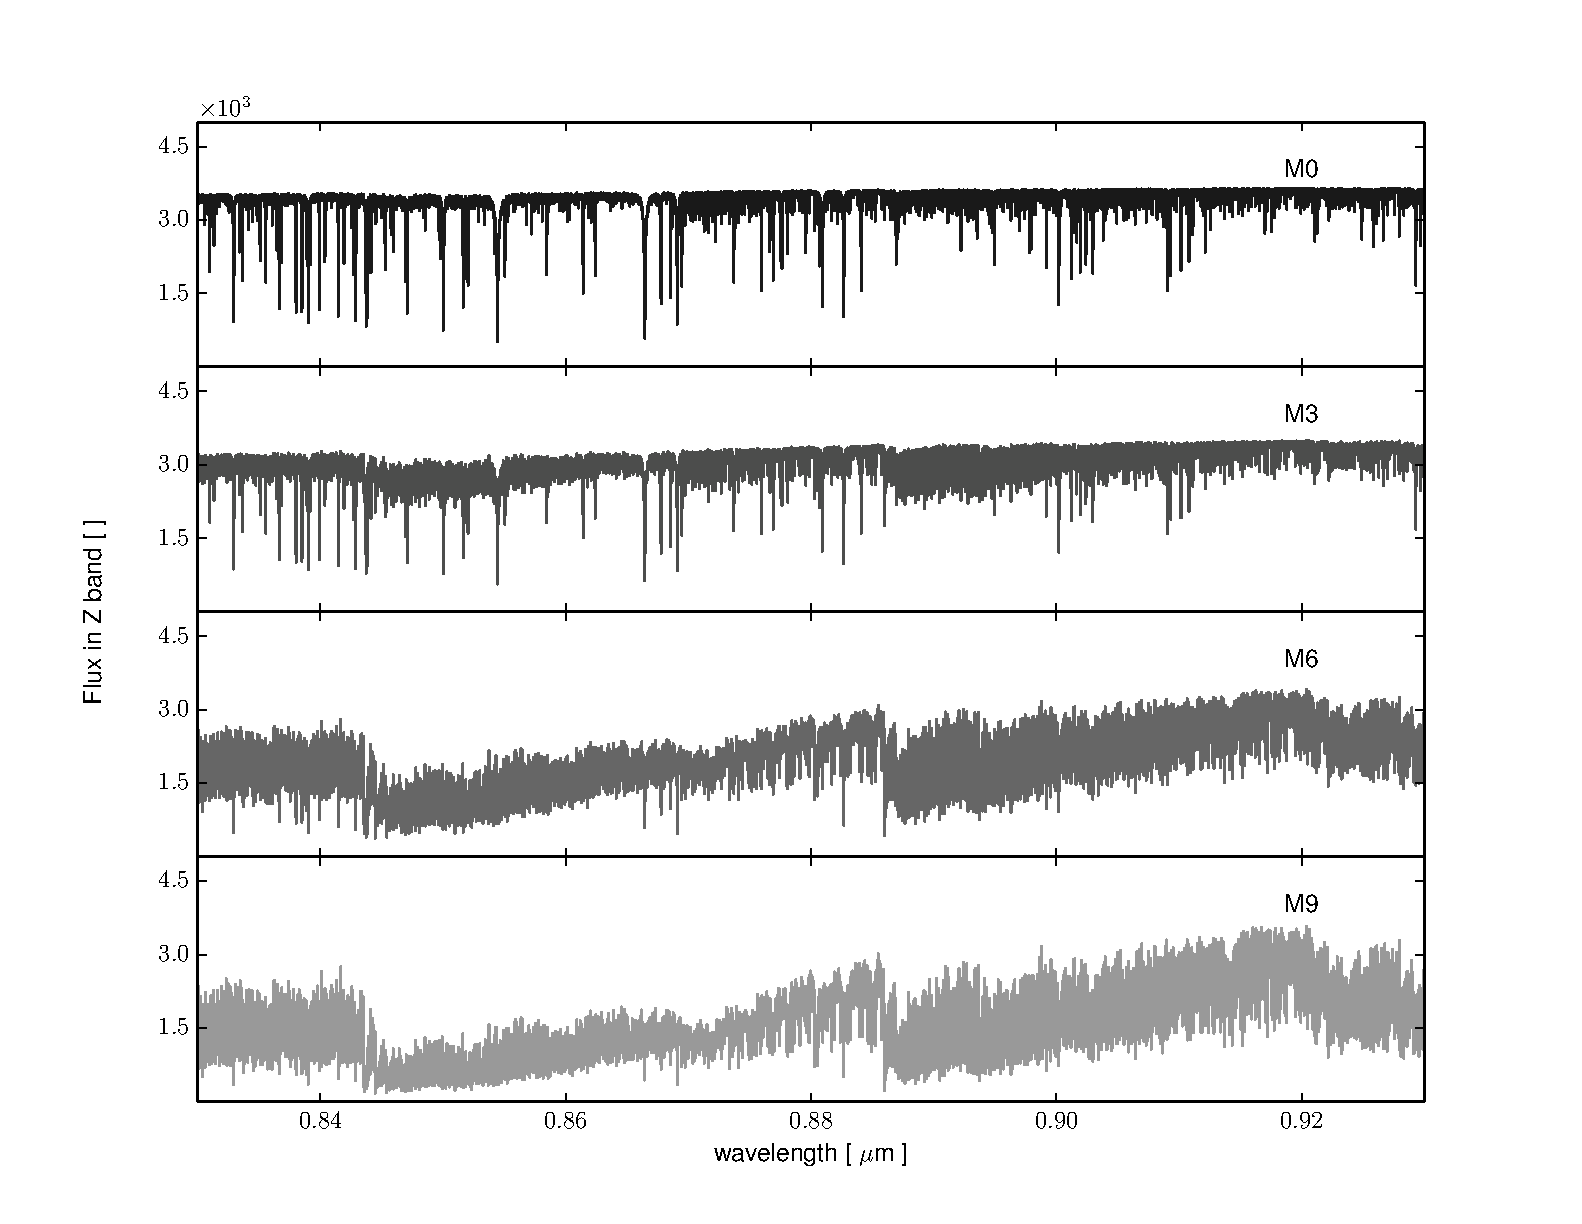
\includegraphics[width=0.9\linewidth]{figures/information-content/figueria_2016_figures/Zband}\\
    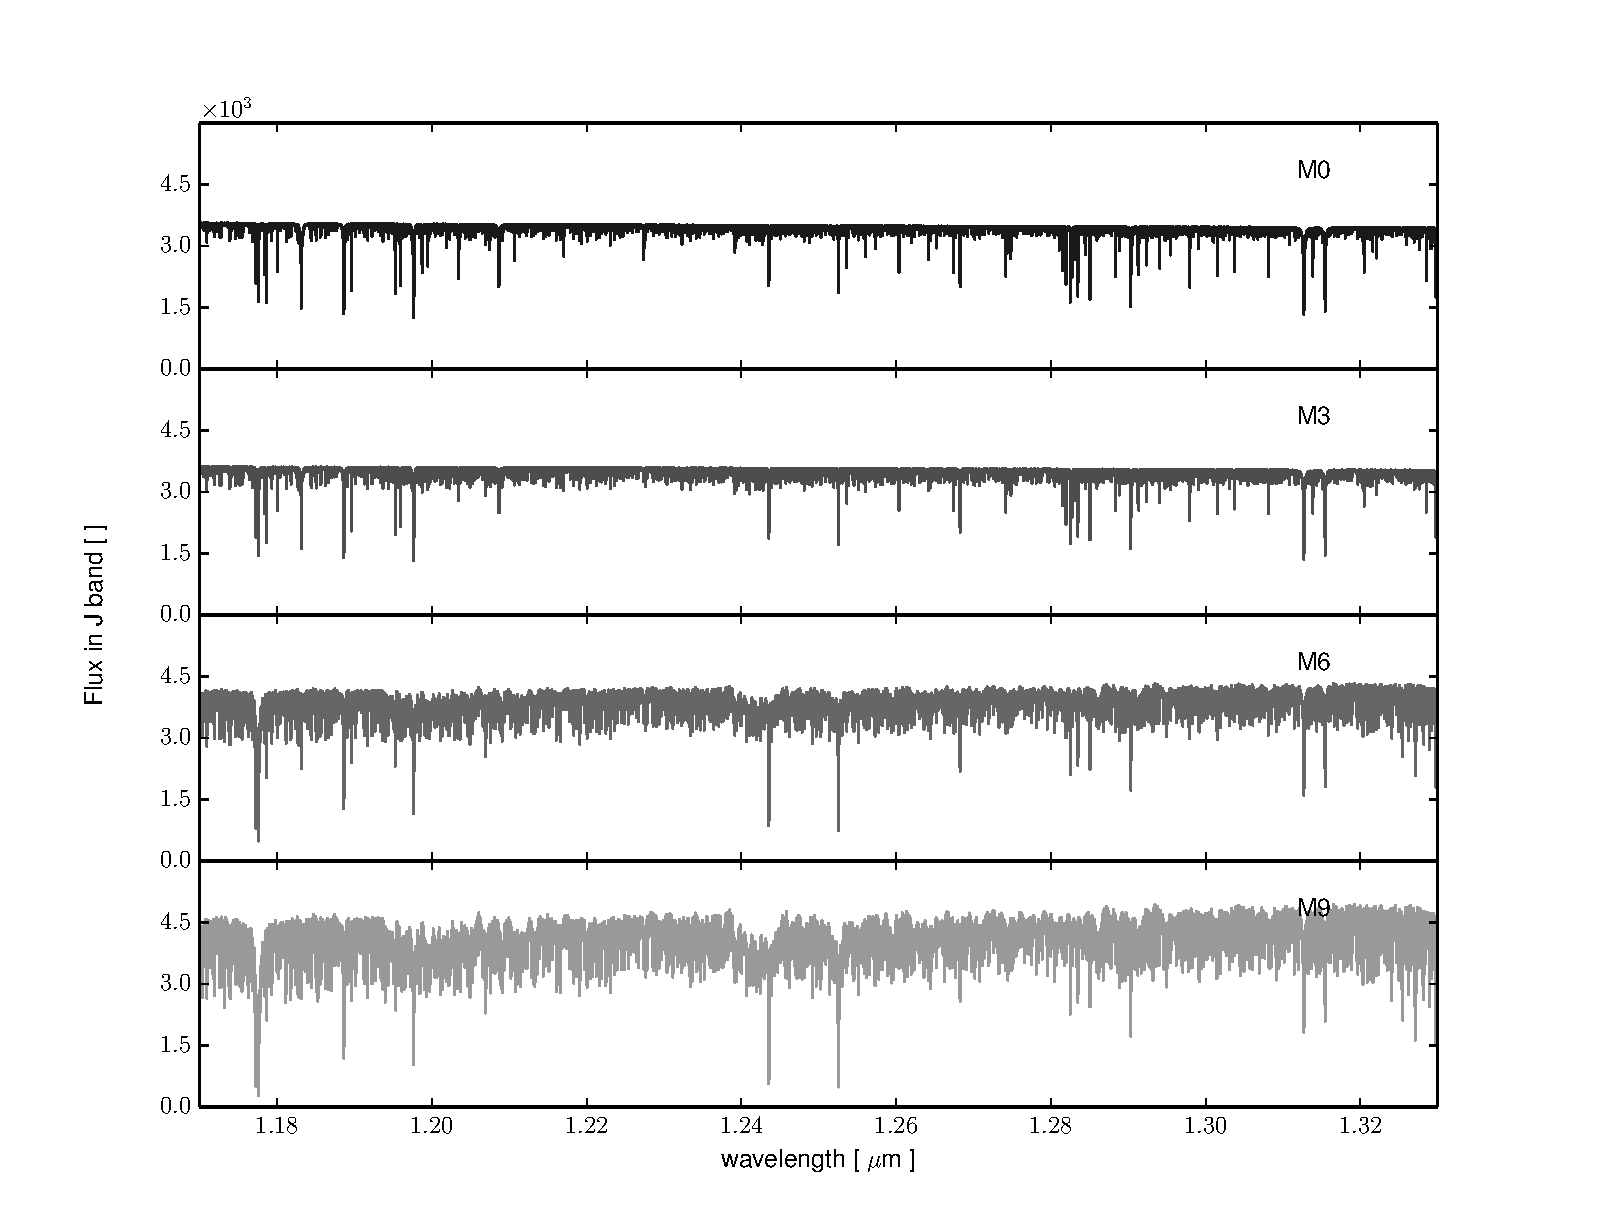
\includegraphics[width=0.9\linewidth]{figures/information-content/figueria_2016_figures/Jband}
    \caption{Flux as a function of wavelength in the \emph{Z}-band (top) and \emph{J}-band (bottom) for the \Vsini{}=1.0\kmps{} and spectral types {M0}, {M3}, {M6}, and {M9} (\textit{top} to \textit{bottom} panels), when seen at a resolution at 100\,000.
        Flux units are arbitrary.
        Reproduced from \citet{figueira_radial_2016}.}
    \label{fig:z_and_j_spectra}
\end{figure}

This work begins to reveal how the spectral parameters \Logg{} and \feh{} begin to affect the {RV} precision obtained.
It shows that there are some fairly consistent trends at the longer wavelength bands, but in the \emph{Z}-, \emph{H}-, and \emph{J}-bands the effect clearly also depends on the spectral type.
This is just the first look into the relationships between \feh{} and \Logg{} in relation to the spectral quality.

With the possibility to simply compute the quality and precision of a large range of synthetic spectral parameters, a comparison of spectral quality over all synthetic spectra or just all in the M-dwarf temperature range, may help solidify or extend the trends observed here. For example, this work has yet assessed the spectral quality when both \feh{} and \Logg{} are changed together.

{\red{}In the context of selecting M-dwarf targets for {RV} measurements, if the goal is to achieve a high spectral quality, then it follows from \cref{fig:logg_metalicity_deviations} that generally for {M0}-M3 spectral types, and in the \emph{H}- and \emph{K}-band, an observation of a metal-rich (\feh{}>0) M-dwarf with a lower \Logg{} value would have a higher spectral quality.
In practise, the spectral quality is only one component to the precision, and probably the  more important, and observer adjustable,  contribution to spectral precision is the number of photons counted (or the \snr{} achieved).
For cool {M6} and {M9} spectral types this is important as longer exposure times are needed to achieve a similar \snr{} level due to their lower luminosity.}\todo{un-red}


\section{{SPIRou} and {NIRPS} {ETC}}
\label{sec:spirou_nirps_etc}
Having \eniric{} as a tool to calculate {RV} precisions efficiently lead to contributions to the Exposure Time Calculators (ETC) for both the {SPIRou} and {NIRPS} spectrographs.
In this way the expected radial velocity precision of the targets can be estimated and provided to those preparing to observe with these spectrographs.
The calculations were performed at the individual request of both instruments.

In September 2017 \eniric{} was used to provide precision calculations for the {SPIRou} ETC\footnote{\url{http://www.cfht.hawaii.edu/Instruments/SPIRou/SPIRou_etc.php}}.
These were the same spectral parameters as~\citet{figueira_radial_2016} except with the precisions for each band referenced to {\snr{}=100} in its own band.
The modification of \cref{subsec:snr_scaling} was made to fulfil this request.
These values are given in \cref{tab:spirou_precisions}.

In May 2018 \eniric{} was used to provide precision calculations for the {NIRPS} {ETC}.
This extended the spectral range from {M0}, {M3}, {M6}, {M9} at 3900, 3500, 2800, 2600\K{} respectively, to all temperatures between 2500\K{} and 4000\K{} inclusively.
This provides a finer resolution coverage over the M spectral type, allowed by the {PHOENIX-ACES} library.
Instrumental resolutions of 75\,000 and 100\,000 were requested to match the {NIRPS} instrument.
The \Logg{}, metallicity, and sampling rate remained at the~\citet{figueira_radial_2016} levels of 4.5, 0.0 and 3.0 respectively.
Precisions were provided for \snr{} of 100 relative to the \emph{J}- and \emph{H}-bands as well as to each band individually.
Artigua (\emph{priv.\ comm.} 2018) suggested the truly relevant values would be the \snr{} in \emph{H}-band for {NIRPS} instrument.
The values calculated for {NIRPS} are given in \cref{tab:nirps_precisions}.

The resulting tables, along with the command line incantations to produce them are detailed in \cref{appendix:nir_prec_amendment}.

\clearpage


%!TEX root = ../../thesis.tex

\section{Application to {CARMENES} spectra}

One of the main reasons for focusing on extending the work of~\citet{figueira_radial_2016} was to analyse the differences in {RV} precision of synthetic spectra and observed \nir{}.
This is important for the community to understand the accuracy of synthetic spectra.
\citet{artigau_optical_2018} recently found band-specific discrepancies in the theoretical precision between real and synthetic \nir{} spectra of Barnard's Star.
In 2018 {CARMENES} openly released a spectral library containing one spectrum for each target in their 324 M-dwarf {RV} survey in~\citet{reiners_carmenes_2018}.
With this they provide details on the empirical \(\delta V_{rms}\) measured during their {RV} processing with their {RV} analysis code, {SERVAL}~\citep{zechmeister_spectrum_2018}, using all available spectra of each target.
Spectra from this library has been used to compare the theoretical precision of observed {CARMENES} spectra to synthetic models, and is still in the preliminary stages, with the progress so far demonstrated here.

\subsection{Target selection}
\label{subsec:carmense_targets}
To analyse the precision in different spectral types, a few specific M-dwarfs were selected.
These were selected from the 324 spectra of the {CARMENES} M-dwarf library from~\citet{reiners_carmenes_2018}\footnote{Available at \href{http://carmenes.cab.inta-csic.es/gto/}{\url{http://carmenes.cab.inta-csic.es/gto/}}.}, along with the achieved \snr{} in the visible and \nir{} spectra.

The spectral library data was downloaded, divided into spectral type and ordered by the stated \nir{} {SNR}, to select targets at the high \snr{} end.
To cover the M-dwarf range, targets were selected near each of the spectral types M0, M3, M6 and M9.
For each spectral type (within $\pm0.5$) two stars are selected that have high {SNR} values. This will give eight spectra over the M-dwarf range to analysis.
One of the two selected targets for the M3 type is Barnard's star which has been analysed extensively in~\citet{artigau_optical_2018}, in particular with CRIRES spectra for the \nir{} domain, allowing for direct comparisons between the two works.
The other criteria used for selection was to select targets with a varied range of \Logg{} and \feh{} values if possible.

The selected targets from the {CARMENES} library are provided in \cref{tab:carmenes_selection_updated}.
The spectral parameters (\Teff{}, \Logg{}, \feh{}) for these targets are from~\citet{passegger_carmenes_2018, rajpurohit_exploring_2018} who performed spectral fits of the {CARMENES} spectra with the {PHOENIX-ACES} and {BT-Settl} models respectively.
The uncertainties in the~\citet{rajpurohit_exploring_2018} parameters are \(\sigma_{\teff{}}\)=100\K{}, \(\sigma_{\logg{}}\)=0.3, and \(\sigma_{\feh{}}\)=0.3 while the uncertainties on the 
\citet{passegger_carmenes_2018} values are \(\sigma_{\teff{}}\)=51\K{}, \(\sigma_{\logg{}}\)=0.07, and \(\sigma_{\feh{}}\)=0.16.
There are gaps in the~\citet{passegger_carmenes_2018} values for stars that have the lower \snr{} levels as they are more difficult to analyse/fit.
Neither one has parameters for Luyten's Star, for which the parameters given are from {SIMBAD}.

\begin{landscape}
    %!TEX root = ../../thesis.tex

\begin{table}[h]
    \centering
    \begin{threeparttable}
        \caption[{CARMENES} targets for {RV} precision analysis.]{Selected {CARMENES} targets with stellar parameters from both~\citet{rajpurohit_exploring_2018} and~\citet{passegger_carmenes_2018}.}
        \begin{tabular}{lllcccccccc}
            %\small
            \toprule
            & & & & & \multicolumn{3}{c}{\citet{rajpurohit_exploring_2018}} & \multicolumn{3}{c}{\citet{passegger_carmenes_2018}} \\
            Karmn & Name & SpT & V & \(\snr{}_{\nir{}}\) & \Teff{} & \Logg{} & \feh{} & \Teff{} & \Logg{} & \feh{} \\
            &  &  & mag &  & \K{} & \si{\centi\metre\per\second\squared} & & \K{} & \si{\centi\metre\per\second\squared} &  \\
            \midrule
            J20533+621 & BD+61 2068     & M0.5 & 8.6  & 257 & 3900          & 5.5 & -0.5           & 3828 & 4.71 & 0.03 \\
            J04290+219 & BD+21 652      & M0.5 & 8.3  & 212 & 4000          & 5.5 & 0.5            & 4194 & 4.59 & 0.20 \\
            J07274+052 & Luyten's Star  & M3.5 & 9.9  & 254 & 3467\tnote{a} & -   & -0.1\tnote{a}  & -    & -    & -    \\
            J17578+046 & Barnard's Star & M3.5 & 9.5  & 236 & 3400          & 5.5 & 0.1            & 3278 & 5.10 & -0.12 \\
            J11055+435 & WX UMa         & M5.5 & 14.5 & 140 & 3000          & 5.5 & 0.3 & - & - & - \\
            J10564+070 & CN Leo         & M6.0 & 13.5 & 133 & 2900          & 5.4 & 0.1 & - & - & - \\
            J18356+329 & LSR J1835+3259 & M8.5 & 18.3 & 50  & 2400          & 5.0 &-0.1 & - & - & - \\
            J04198+425 & LSR J0419+4233 & M8.5 & 11.1 & 42  & 2400          & 4.9 & 0.1 & - & - & - \\
        \bottomrule
        \end{tabular}\label{tab:carmenes_selection_updated}
        \begin{tablenotes}
            \item [a] {From SIMBAD.}
        \end{tablenotes}
    \end{threeparttable}
\end{table}

\end{landscape}


\subsubsection{Spectral preparation and Telluric correction}
\label{subsec:prepatation_on_carmenes}
The spectra in the  {CARMENES} library have not been corrected for telluic lines.
To properly assess the theoretical {RV} precision attainable in the {CARMENES} spectra they need to be corrected for telluic lines.
Telluric correction is performed with the {Molecfit} software~\citep{smette_molecfit_2015} in collaboration with Sol\'ene Ulmer-moll, who has {Molecfit} experience~\citep{ulmer-moll_telluric_2018}.

The separate spectral orders first need to be combined into a single spectrum.
At this stage, where spectral orders overlap only the flux from one order is kept for simplicity.
The overlapping regions could be combined by taking the mean because the overlapping orders are well aligned in wavelength, but this was not performed at this exploratory stage.

The telluric correction is performed by dividing the {CARMENES} spectrum by a telluric transmission spectrum fitted with {Molecfit}.
The fitting with {Molecfit} has been attempted two different ways.
The first correction performs the fitting on the full \nir{} spectrum, while the second splits the spectrum into three parts and fits them separately.
This was done because it was noticed that the spectral line shape changes significantly from 0.9\um{} to 1.7\um{}.

Different molecules are fitted in the three separate parts.
In the first part (0.9--1.1\um{}) \ce{H2O} is fitted, in the second (1.1--1.5\um{}) \ce{O2} is fitted while \ce{CO2} and \ce{CH4} are fitted in the third section (1.5--1.71\um{}).
After this all molecule abundances are fixed and the final fit is performed on each of the three parts.

In the end, splitting the spectrum into three does not seem to improve the telluric correction considerably.
The telluric spectrum fitted from both attempts is shown in the top panel of \cref{fig:compare_telluric_corrections}.
The difference between the two telluric spectra changes is shown in the bottom panel.

It is unknown whether the full telluric correction of the {CARMENES} \nir{} spectrum has been performed before.
There has been one publication known which uses {Molecfit} to correct a {CARMENES} spectrum, but only in a very narrow spectral range (1.082--1.084\um{})~\citep{allart_spectrally_2018}.
As such there is not yet a definitive guide to achieve the best telluric correction of {CARMENES} spectra with {Molecfit}.

In this work only one spectrum has been telluric corrected to compare the difference between the two {Molecfit} corrections and their improvement over complete telluric masking on spectral quality and {RV} precision.
This was to see if it is worth investing time to improve the telluric correction step.

After telluric correction the spectrum was corrected for bad pixels by linear interpolation across them.
Some examples of bad pixels can be seen in a narrow wavelength range in \cref{fig:carmenes_spike_removal}.
The lines with orange circles and green crosses are the original and telluric corrected spectra, respectively.
They both show individual bad pixel spikes throughout the spectrum.
The black line is the spectrum corrected from the bad pixels (labelled `fixed') for the bad pixels. 
The blue line is a ``quality flag'' output (0 or 1) from {Molecfit}, indicating where the spectrum has a flux below or equal to zero.
It correctly identifies one of the bad pixels but not the others that have a flux above zero.
Within the \emph{Y}- \emph{J}-, and \emph{H}-bands there are around 213/66069\(\sim\)0.3\% bad pixels identified with an automated algorithm, based on a maximum derivative threshold (the bad pixels have very high derivatives).

The removal of bad pixels, which introduce pixels with very high derivatives (and pixel weight, $W(i)$), is essential for an accurate computation of the spectral quality and RV precision.
The sharp lines with high derivatives would artificially increases the calculated spectral quality, \(Q\), masquerading as very deep and narrow spectral lines.

\begin{figure}
    \centering
    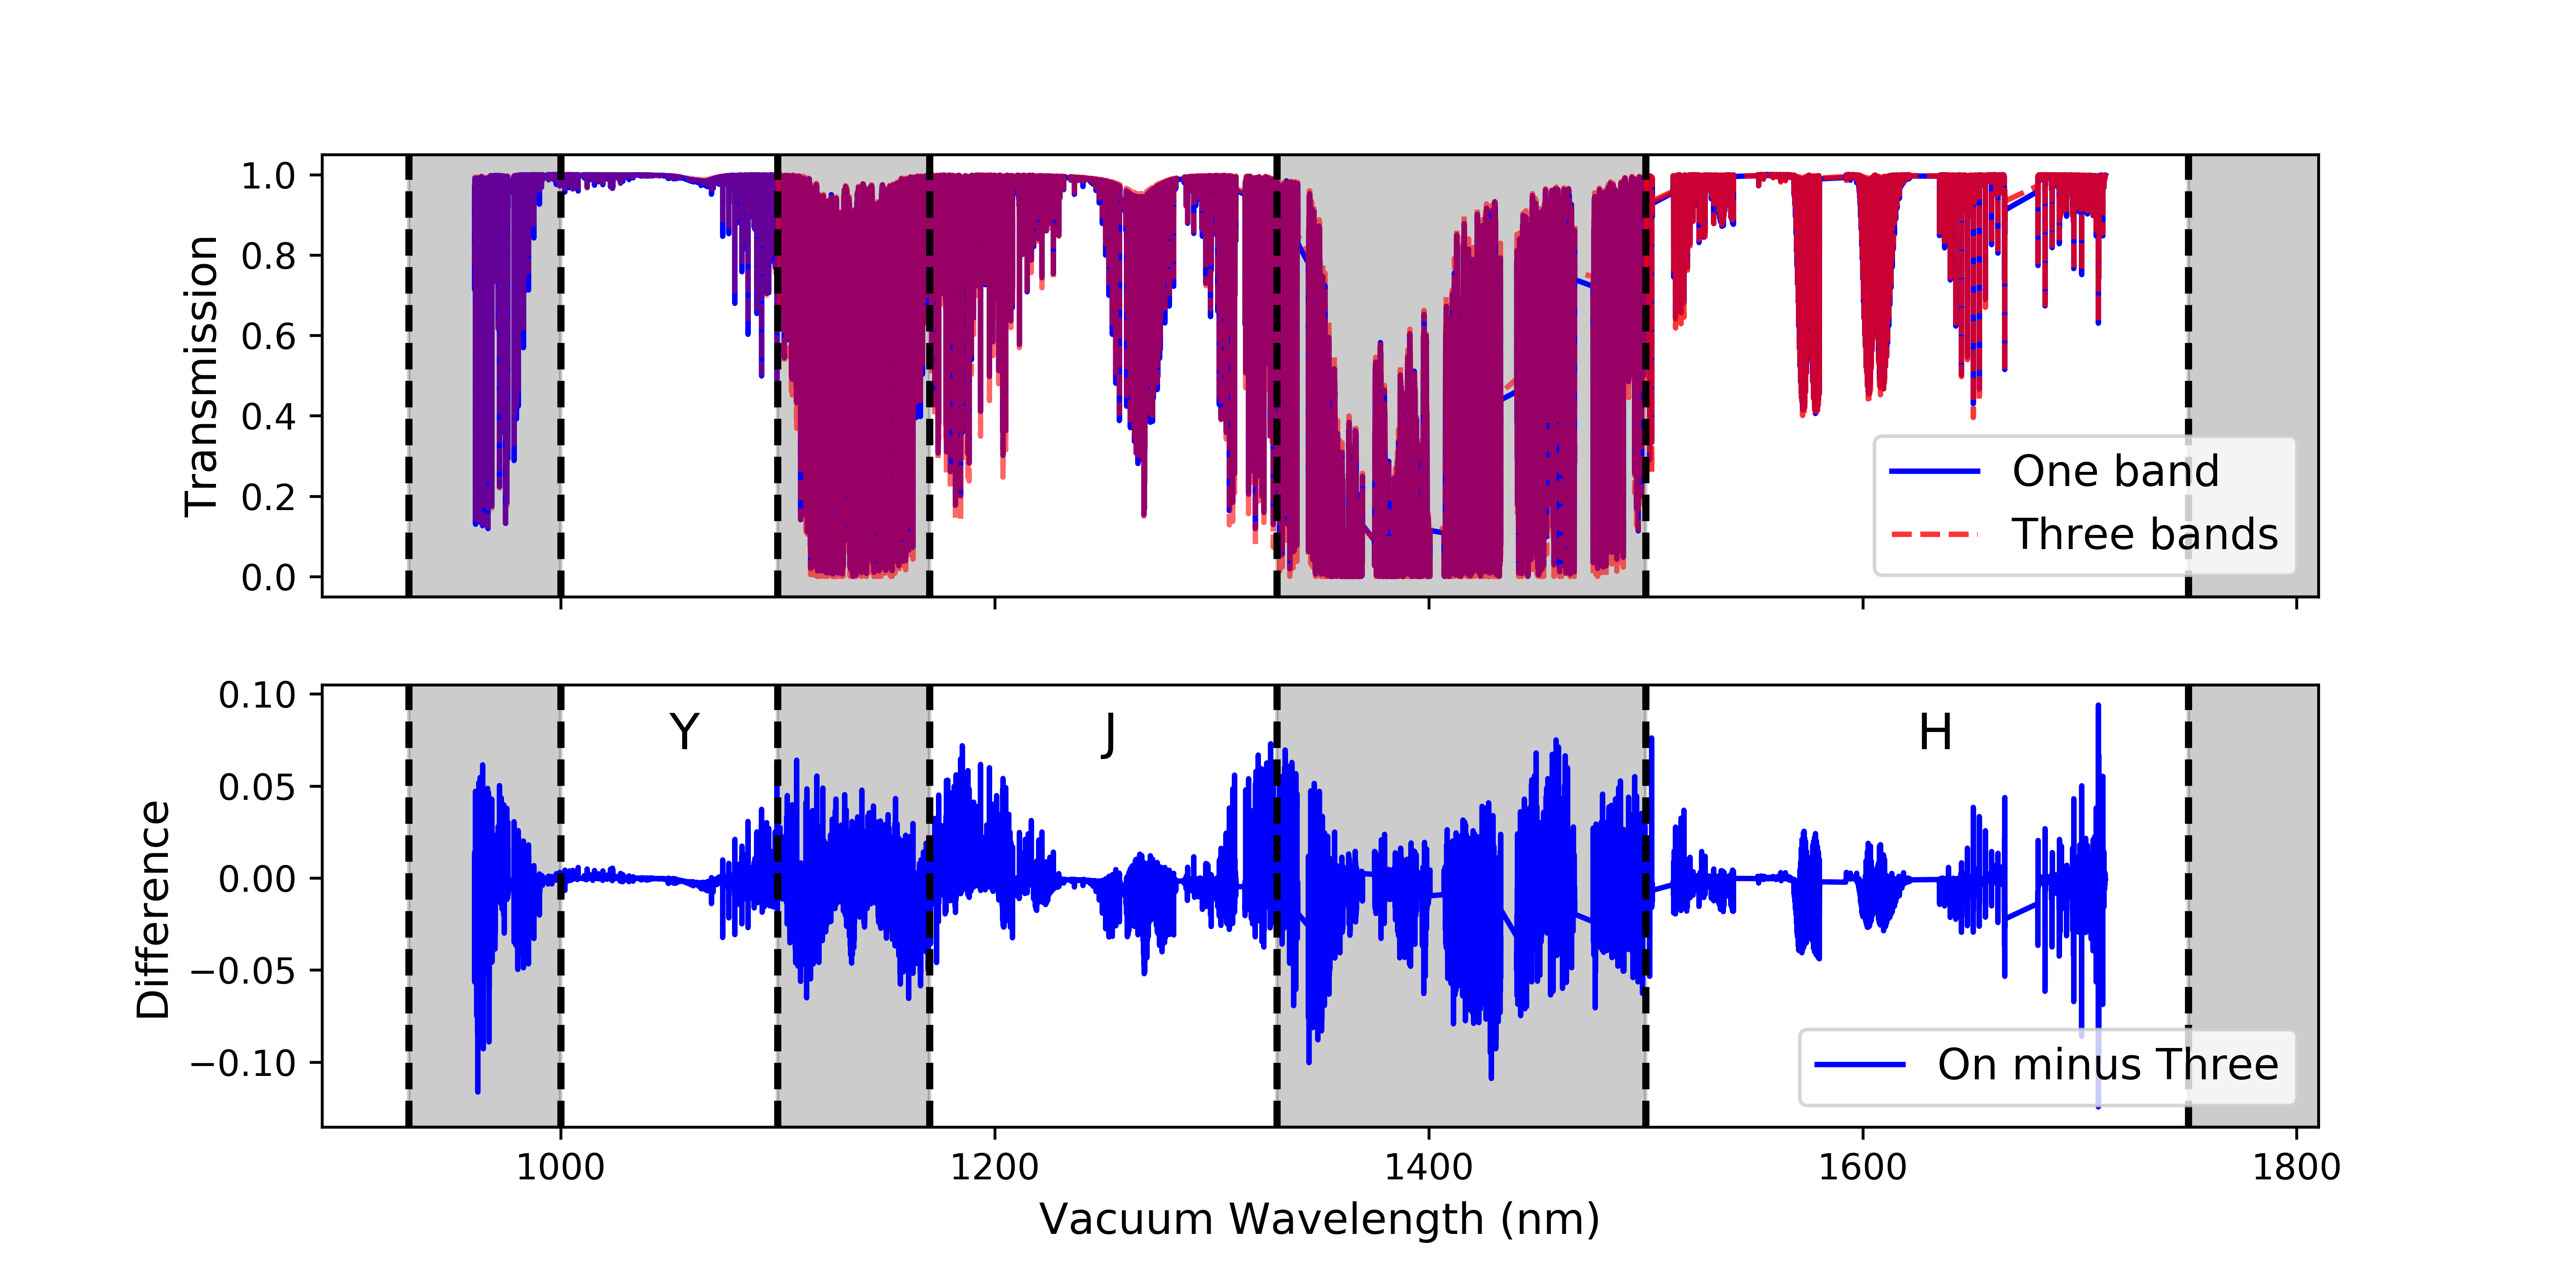
\includegraphics[width=0.9\linewidth]{figures/information-content/Carmenes/compare_telluric_corrections_shaded}
    \caption[]{Comparison of telluric models in pursuit of a better correction.
        Top: The two synthetic telluric spectra.
        The blue shows the result from {Molecfit} after treating the full spectrum as one, with a single spectral profile, while the shaded red telluric spectrum has been derived with three separate bands, fitted individually.
        Bottom: The difference in the telluric spectrum between the fit to the full spectrum, and the fit with the spectrum split into three.
        The regions of deep \ce{H2O} absorption lines which defined the \nir{} bands are shaded grey.
        The bounds of each band from \cref{tab:infrared_bands} are indicated with vertical black dashed lines.}
    \label{fig:compare_telluric_corrections}
\end{figure}


\begin{figure}
    \centering
    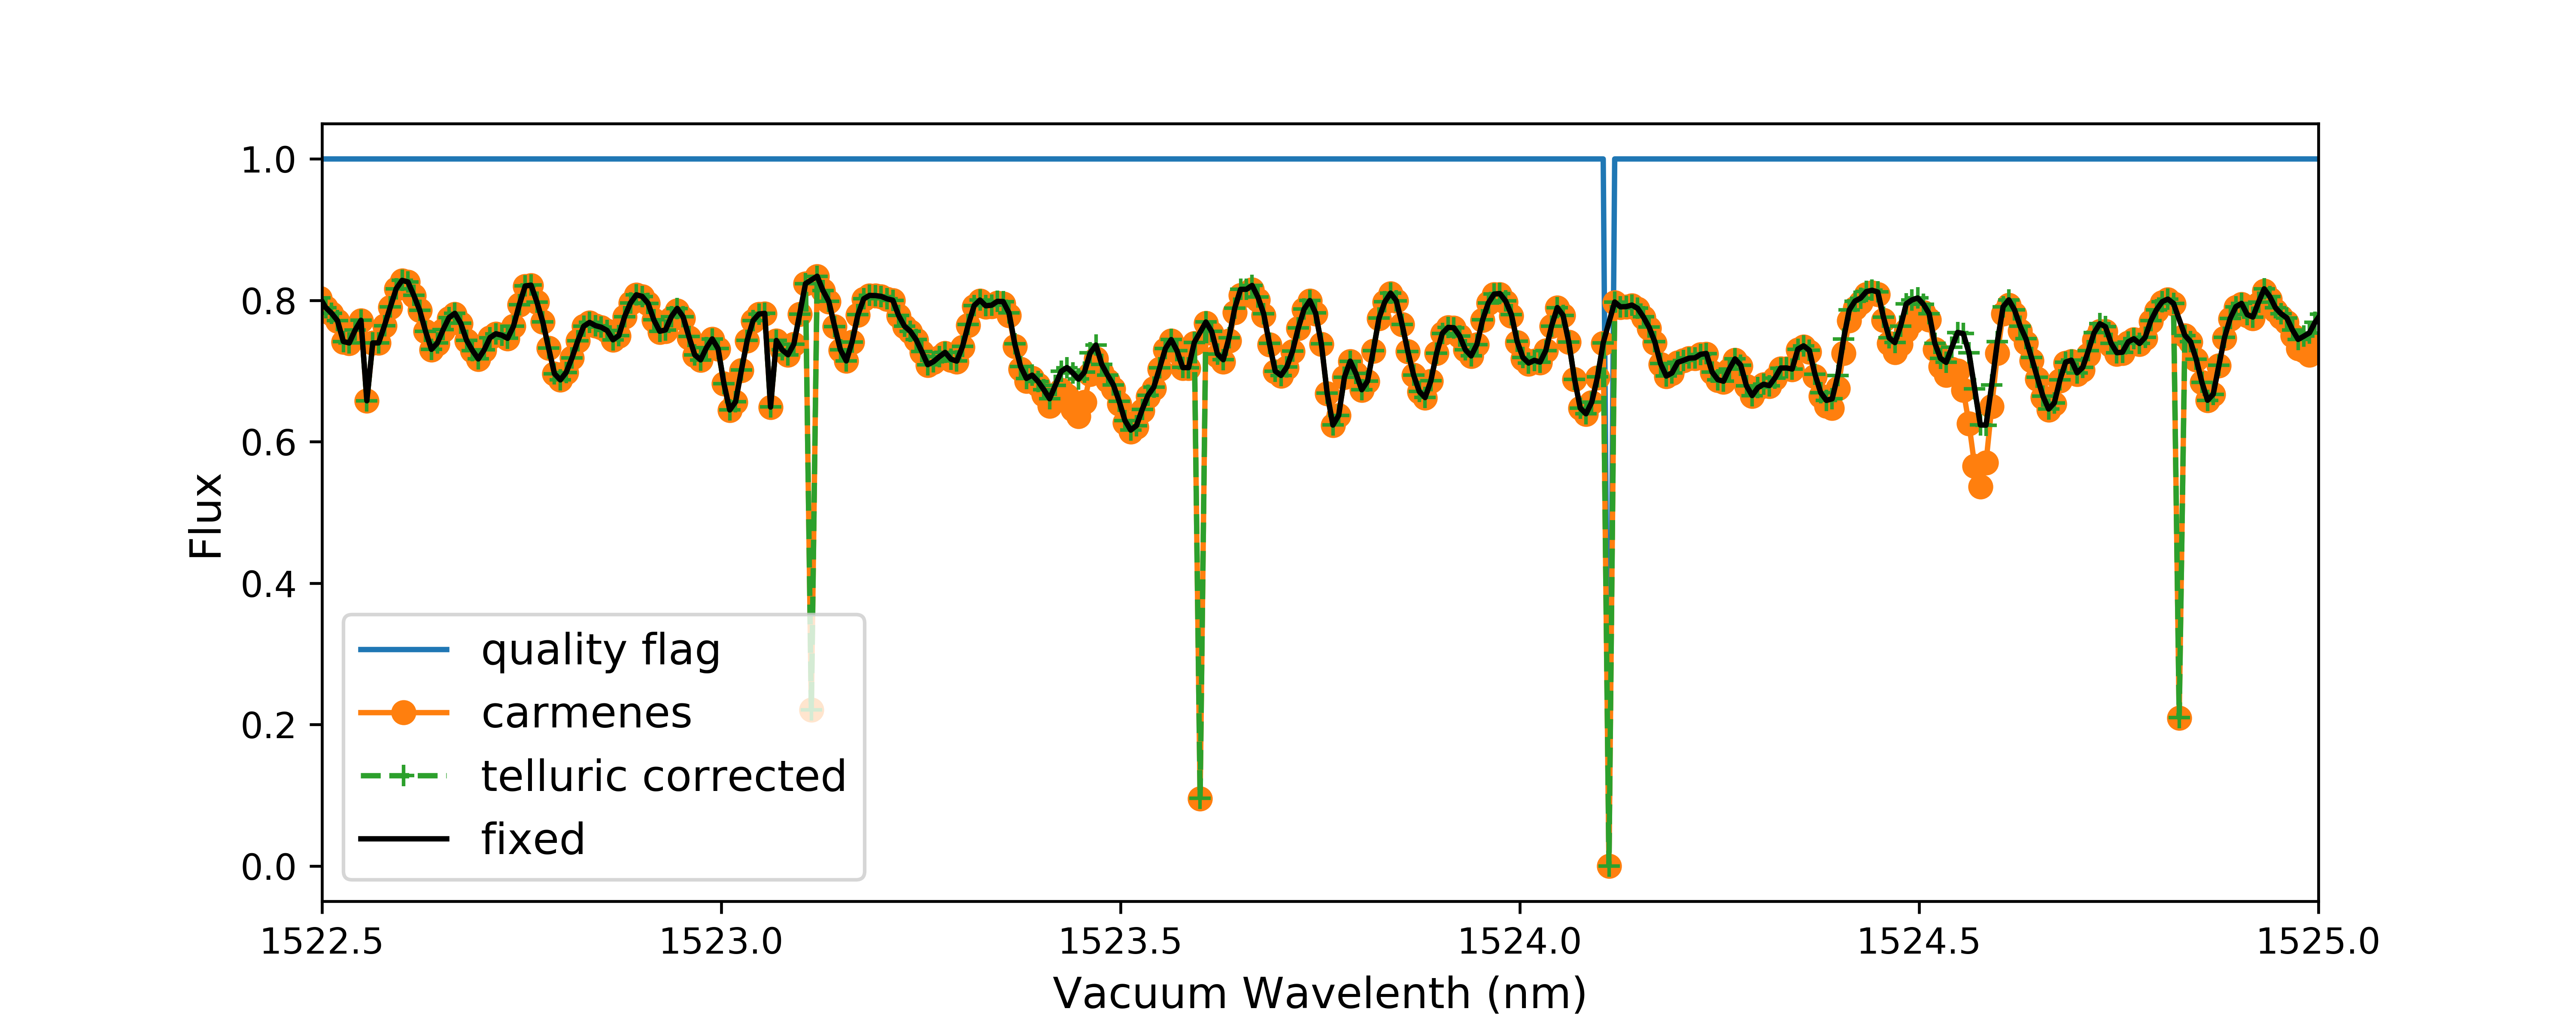
\includegraphics[width=0.9\linewidth]{figures/information-content/Carmenes/carmenes_spike_removal}
    \caption[Bad pixel removal in {CARMENES}.]{Removal of bad pixels from the {CARMENES} spectrum. The orange line with circles and green line with pluses are the original and telluric corrected spectra from {CARMENES}.
    The black solid line shows the spectrum after correction from bad pixels.
    The blue line shows the ``quality flag'' (0 or 1) output from the {Molecfit} software.}
    \label{fig:carmenes_spike_removal}
\end{figure}


\subsection{Impact of telluric correction}
\label{subsec:impact_telluric_correction}
Here the impact of the telluric correction on the spectral quality of the CARMENES spectrum is assessed.
This was done by calculating, Q, with the original telluric lines deeper than 2\% masked out, and with the telluric correction performed.
This was done for both fitting methods attempted with Molecfit and displayed in \cref{fig:band_qualityfromapplyingtelluriccorrection}.
The top panel shows the telluric corrected spectrum (orange) along with the telluric mask that was applied (blue).
The bottom panel shows the spectral quality for the three spectral bands \emph{Y}, \emph{J}, and \emph{H}.

\begin{figure}
    \centering
    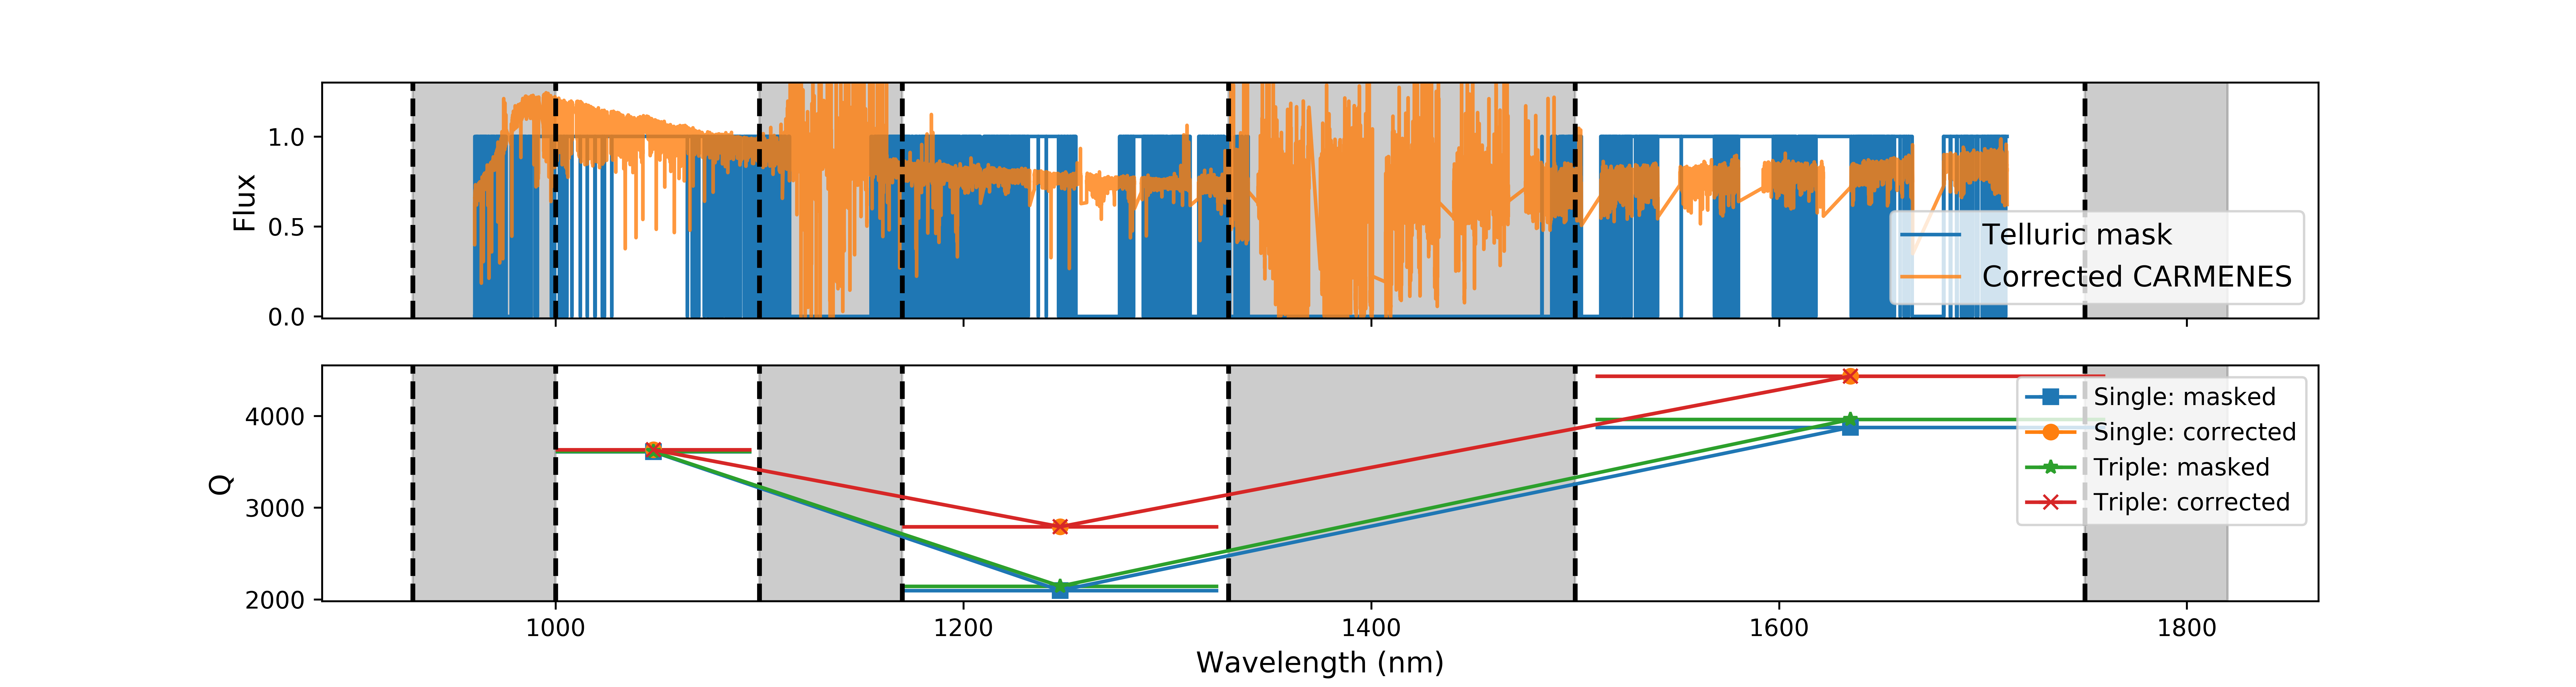
\includegraphics[width=0.8\linewidth]{figures/information-content/Carmenes/Band_quality_from_applying_telluric_correction}
    \caption[Barnard's star spectral quality.]{Measured spectral quality, Q, in the three \nir{} bands of Barnard's star to assess the gain from telluric correction. 
        Top: The telluric corrected CARMENES spectrum (orange) along with the binary mask for telluric lines >2\% depth (blue). 
        Bottom: The spectral quality in the three spectral bands, for different telluric treatment. `single' indicates the Molecfit results from the single fit to the spectrum, while `triple' indicates the fit to the three wavelength bands.
        `masked' indicates that telluric masking of the lines deeper than 2\% was performed and while `corrected' is just the telluric corrected spectrum.}
    \label{fig:band_qualityfromapplyingtelluriccorrection}
\end{figure}

\cref{fig:band_qualityfromapplyingtelluriccorrection} shows that there is a benefit (gain in quality) from telluric correction in the \emph{J} and \emph{H}-bands, where there are numerous telluric lines.
However, in the \emph{Y}-band where there is little telluric masking performed there is only a slight gain.
Performing telluric correction of the CARMENES spectra over telluric masking causes a gain the the spectral quality by 1\%, 30\%, 12\% in the \emph{Y}-band, \emph{J}, and \emph{H}-bands respectively.
As the spectral quality is related to the RV precision, this will lead to a 10-30\% improvement in the RV precision in the \emph{J}- and \emph{H}-bands
This indicated that it is worth performing telluric correction on the other seven {CARMENES} targets selected.
This also shows that the extra effort from three separate telluric fittings does not lead to a significant gain in quality.


\subsection{Barnard's star}
\label{sec:carmenes_barnards_star}
Currently only Barnard's star has had the telluric correction performed, and as such the analysis for this target is shown.
The spectral content of Barnard's star was extensively explored in~\citet{artigau_optical_2018} comparing the synthetic model to observations from {HARPS}, {ESPaDOns} and {CRIRES} in the range 380--2300\nm{}.
Agreement was found in the optical but the \nir{} bands had significant differences between the observations and models. 
The goal of this analysis is to check if the same results are obtainable in the {CARMENES} spectrum of Barnard's star.

\citet{artigau_optical_2018} tabulated several literature values for the stellar properties of Barnard's star and identified the closest matching {PHOENIX-ACES} model.
The synthetic model adopted for Barnard's star was \Teff=3200\K{}, \Logg{}=5.0, and \feh{}=-0.5, and we adopt the same model here.
This is tabulated in with other parameters from~\citet{artigau_optical_2018} in \cref{tab:barnards_star_params}.

\begin{table}
    \centering
    \caption[Properties of Barnard's star.]{Properties of Barnard's star from~\citet{artigau_optical_2018}. \Teff{}, \feh{} and \Logg{} values are only the adopted (closest) model parameters.}
    \begin{tabular}{lc}
        \toprule
        Parameter & Value \\
        \midrule
        SpType & M4\,Ve \\
        Rotation Period & \(\sim\)130 days \\
        \Vsini{} & \(\le 80\) \si{\metre\per\second} \\
        \Teff{} & 3200 \K{} \\
        \Logg{} & 5.0 \\
        \feh{} & -0.5 \\
        \bottomrule{}
    \end{tabular}\label{tab:barnards_star_params}
\end{table}

A series of spectra are shown in \cref{fig:carmenes_correction}.
The uncorrected {CARMENES} spectrum of Barnard's Star is shown in the first panel.
The second panel shows telluric model from Molecfit, while the third panel shows the telluric corrected spectrum.
In the telluric corrected spectrum there are several deep spikes which are bad pixels.
Most of these are corrected for in the fourth panel, although it appears there may be a few still present in the spectrum.
The fifth panel contains the synthetic PHOENIX-ACES spectrum of Barnard's star, used to compare the spectral quality.
The model has been convolved by an instrumental profile with R=80\,400, but not rotationally broadened since the \Vsini{} is low. The flux units of the spectra are arbitrary, and the synthetic model has been converted into photon counts.

\begin{figure}
    \centering
    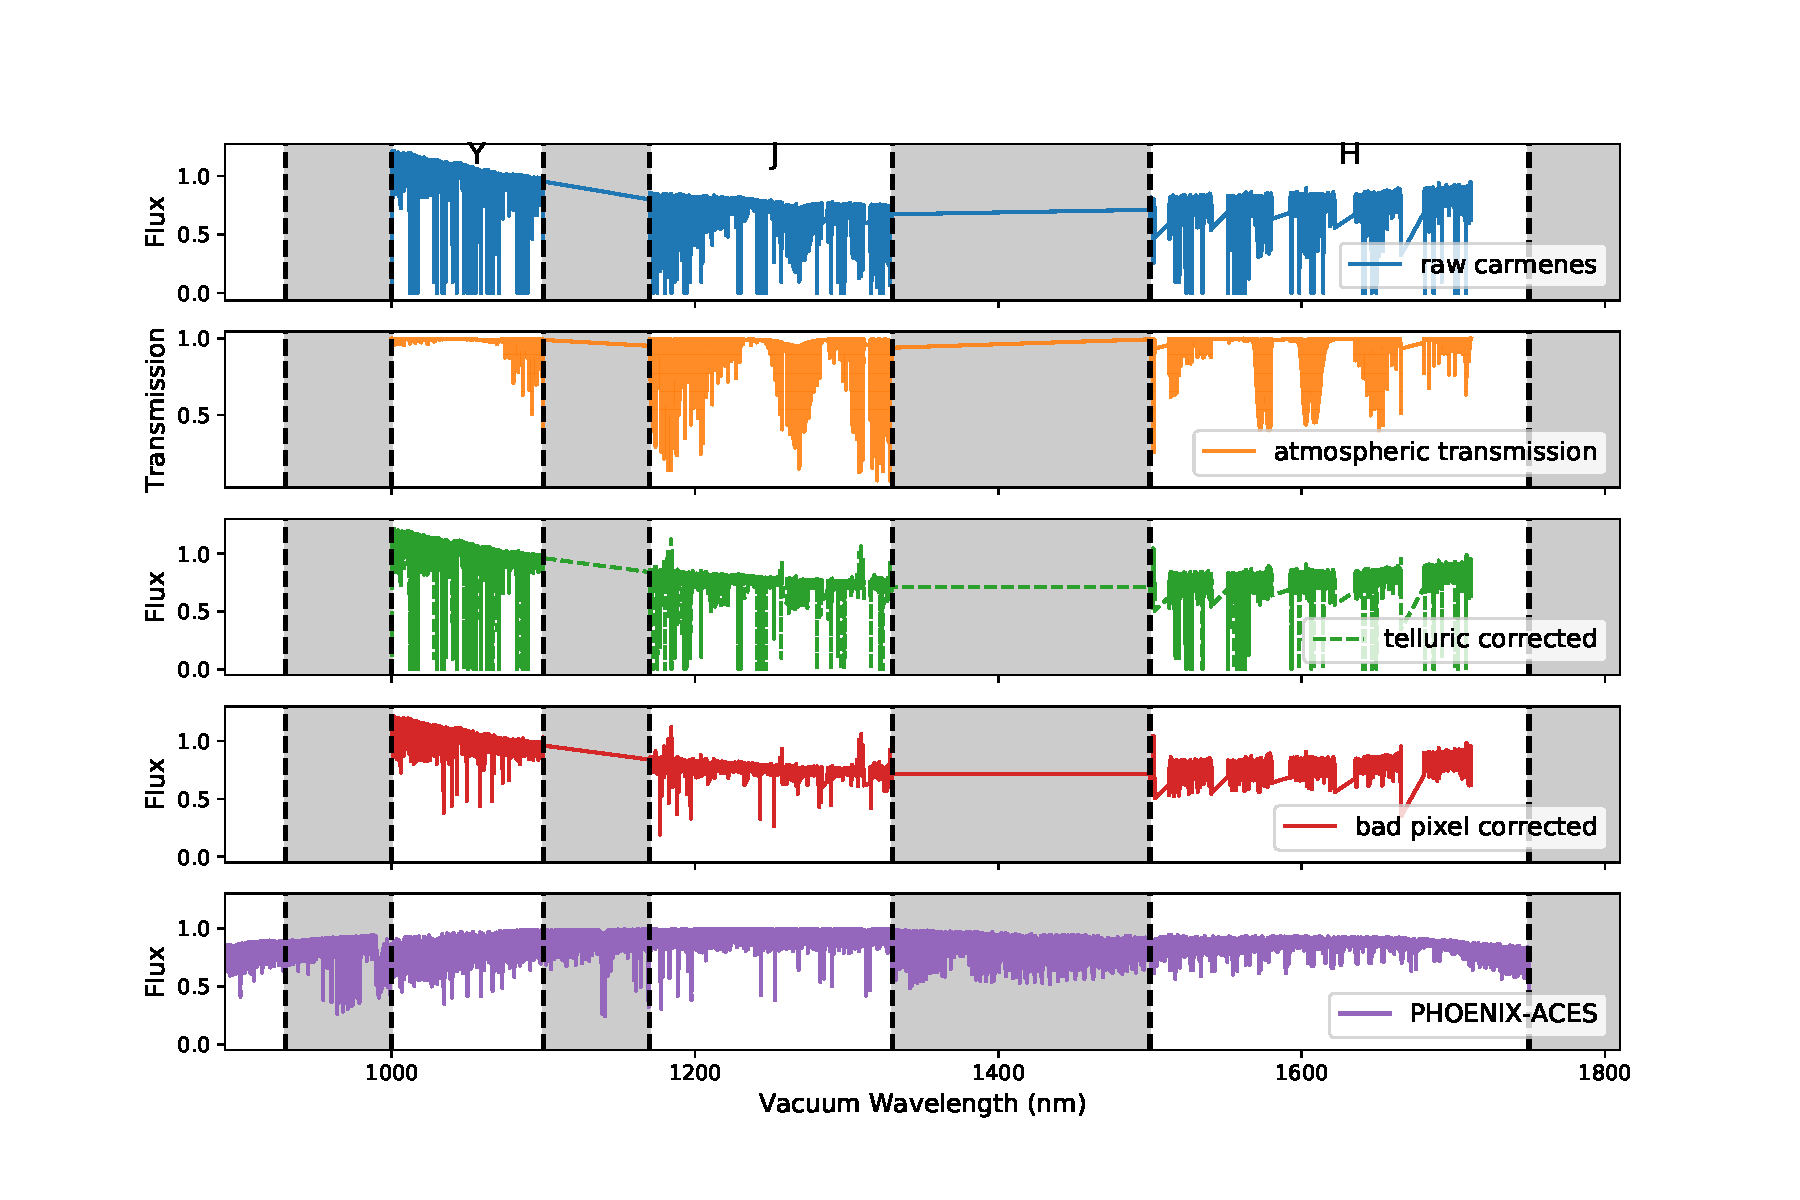
\includegraphics[width=0.8\linewidth]{figures/information-content/Carmenes/bp_carmenes_masked_model_broadened}
    \caption[Telluic correction of the {CARMENES} \nir{} spectrum.]{Telluic correction of the {CARMENES} \nir{} spectrum.
        First: Uncorrected spectrum of Barnard's Star between 960--1710\nm{} from {CARMENES}.
        Second: The synthetic telluric transmission spectrum fitted with {Molecfit}.
        Third: Telluric corrected spectrum by division of the telluric spectrum.
        The regions of deep \ce{H2O} absorption lines which defined the \nir{} bands are shaded grey.
        Fourth: The telluric corrected spectra after the bad pixels are removed.
        Fifth: Synthetic PHOENIX-ACES model for Barnard's star, convolved to R=80\,400.
        The bounds of each band from \cref{tab:infrared_bands} are indicated with vertical black dashed lines.
        The flux units of the spectra are arbitrary}
    \label{fig:carmenes_correction}
\end{figure}


To compare the model to the observation it is interpolated to the pixel positions of the {CARMENES} spectrum.
The spectral quality is calculated for both on small wavelength bins with a width 0.2\% the central wavelength similar to~\citet{artigau_optical_2018}.
The top panel of \cref{fig:qualitycomparisiontomodel} shows the results of the comparison, with the spectral quality in 0.2\%\,\(\lambda\) width bins for the observation (orange squares) and the model (blue stars) in the top panel.
The ratio between the spectral quality of the observation and the model is given in the bottom panel.
It shows that in this instance the \emph{Y}- and \emph{J}-bands have a similar spectral quality, while there is a large difference in the \emph{H}-band with the CARMENES observation having a spectral quality 3--4\(\times\) greater than the model.

\begin{figure}
    \centering
    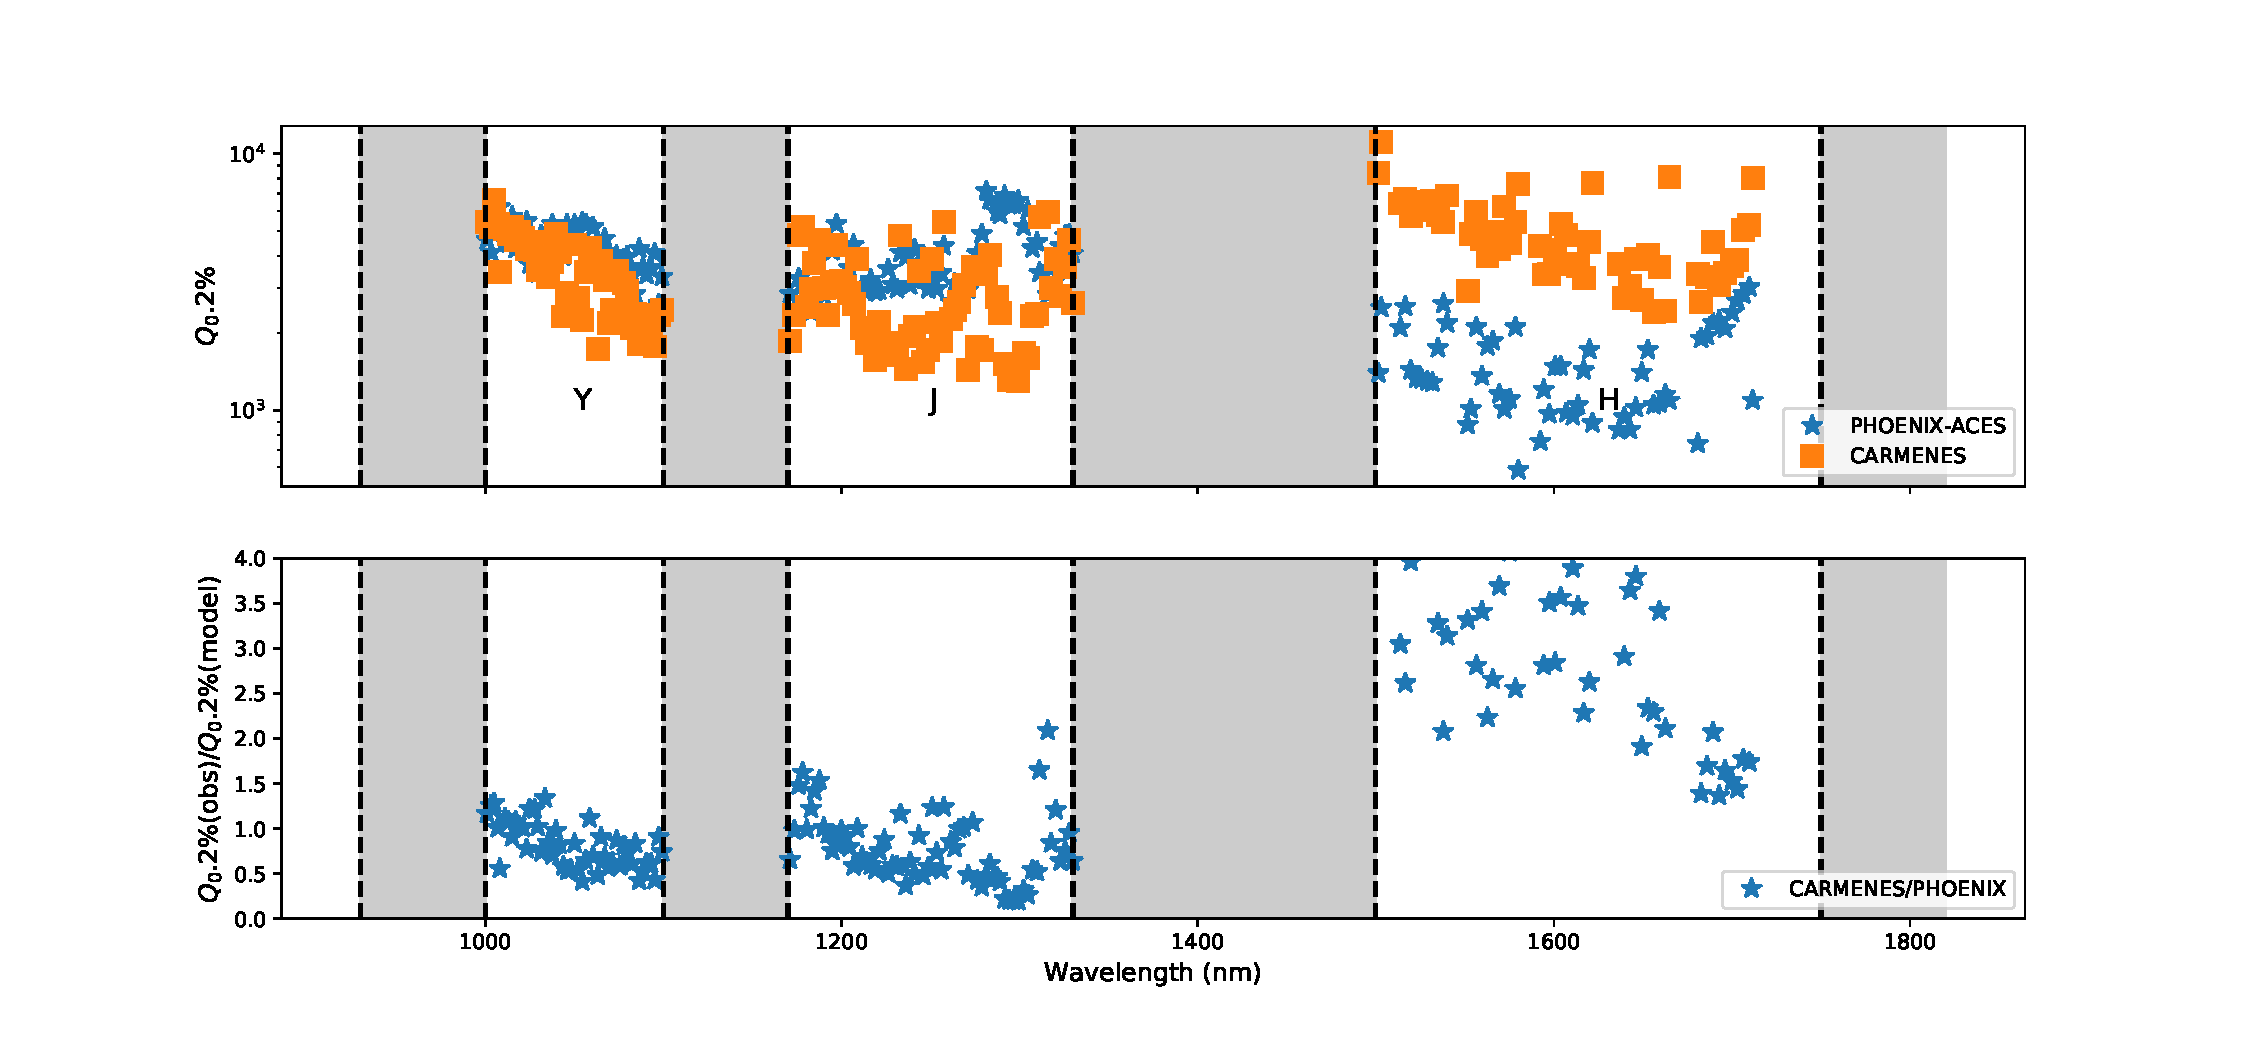
\includegraphics[width=0.8\linewidth]{figures/information-content/Carmenes/quality_comparision_to_model}
    \caption[Barnard's star spectral quality compared to CARMENES.]{Measured RV content of Barnard's star over the near-infrared domain, from CARMENES.
    Top: The spectral quality in 0.2\%\,\(\lambda\) width bins for CARMENES (orange squares) and the model (blue stars).
    Bottom: The ratio of spectral quality observed/model.}
    \label{fig:qualitycomparisiontomodel}
\end{figure}

For comparison the corresponding image from~\citet{artigau_optical_2018} is provided in \cref{fig:allw2}.
It shows a lower computed spectral quality (50\%) in the \emph{Y}- and \emph{J}-bands compared to the model of Barnard's star.
However in this work the model and observation have a similar spectral quality in these bands, although the ratio does drop to 50\% towards the red end of the \emph{J}-band.
In the \emph{H}-band of both works the observed quality is higher then the model, however the CARMENES spectral quality is 3\(\times\) higher, instead of only 1.5\(\times\) in~\citet{artigau_optical_2018}.
This is a significant difference.

\citet{artigau_optical_2018} only apply telluric masking in their analysis, whereas here the telluric corrected spectra were used.
This could be part of the reason for the largely improved results in the \emph{H}.
As shown in \cref{subsec:impact_telluric_correction} the telluric correction can improve the quality by 12--30\%.
However, this does not fully explain the increase by a factor of 2.
This requires further investigation.


\begin{figure}
    \centering
    \begin{tabular}{c}
    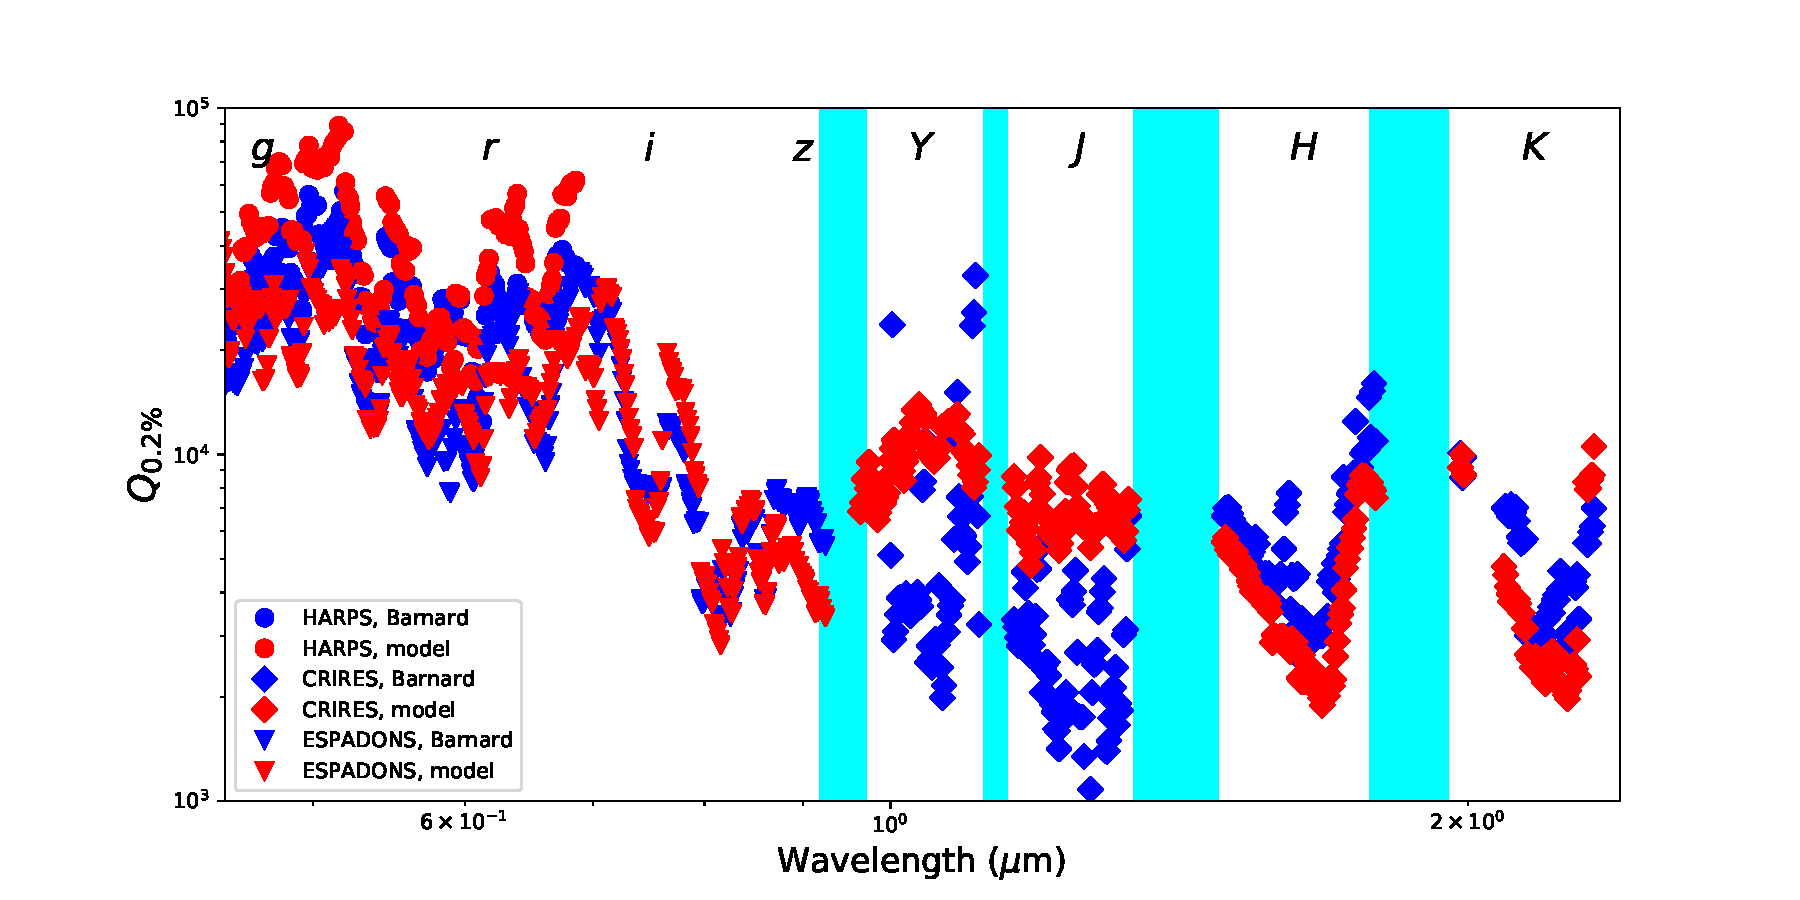
\includegraphics[width=0.8\linewidth]{figures/information-content/artigau2018_figures/all_w}\\
    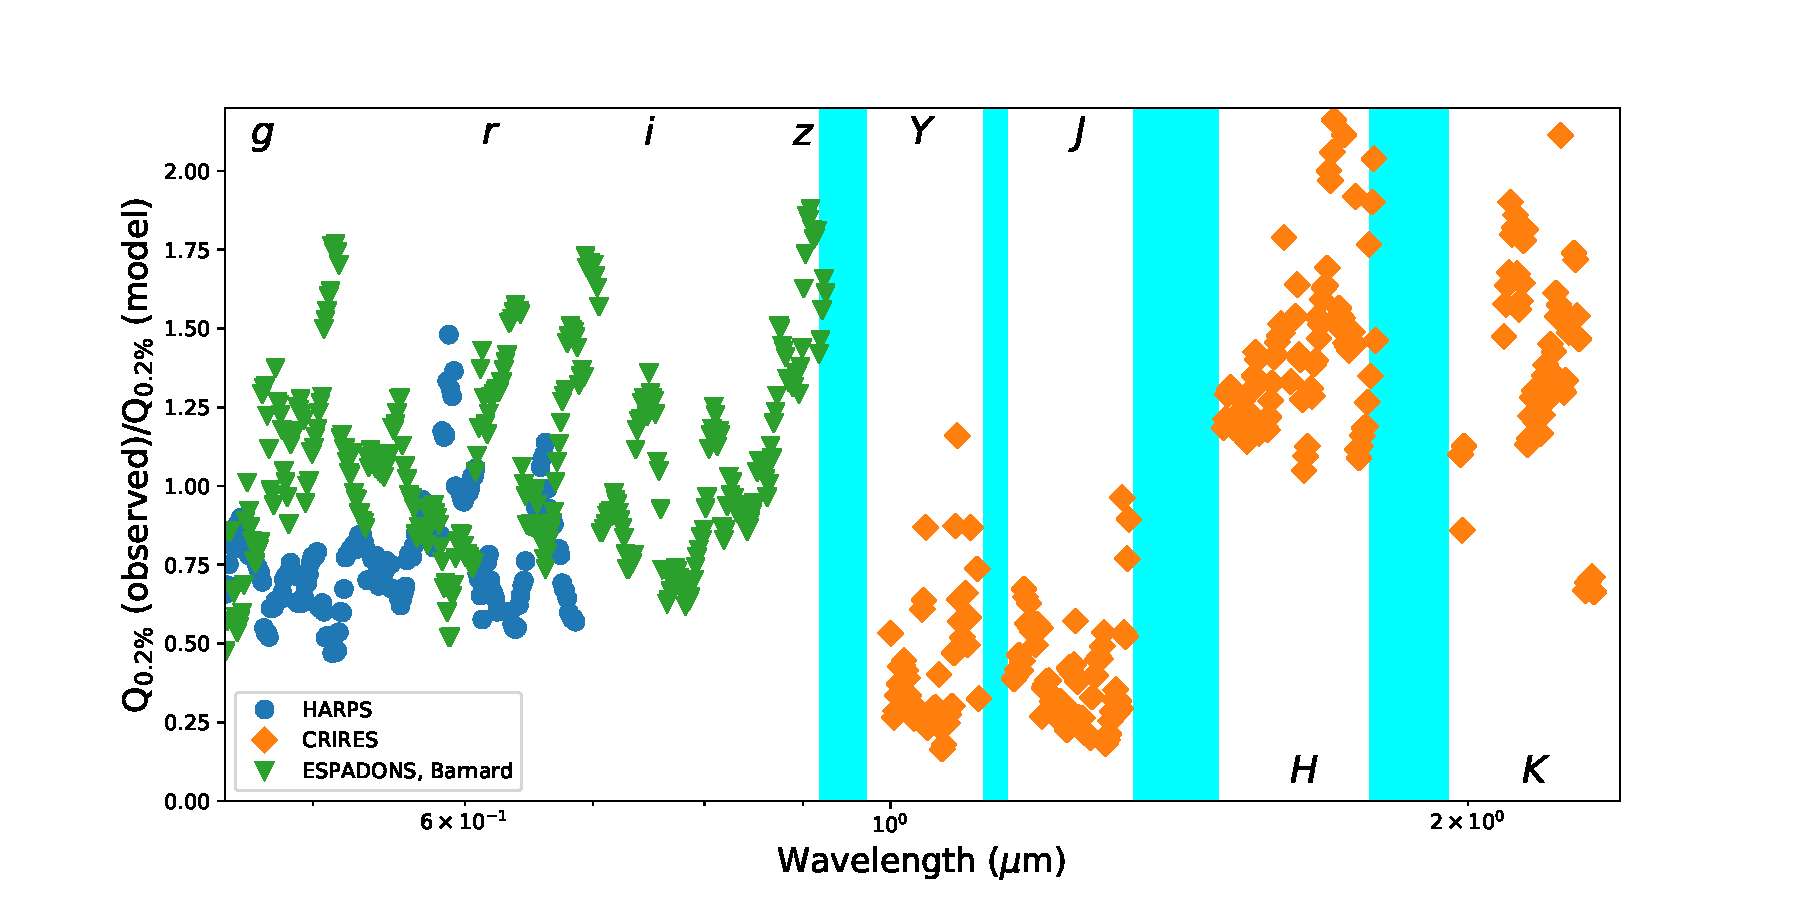
\includegraphics[width=0.8\linewidth]{figures/information-content/artigau2018_figures/all_w2}
    \end{tabular}
    \caption[Measured RV content of Barnard's star over the optical and near-infrared domain.]{Measured RV content of Barnard's star over the optical and near-infrared domain. Overall measured (blue) and model (red) RV density are well matched blueward of $\sim1\mu$m. The agreement is poorer in the near-infrared domain with an over-prediction of RV content in $Y$ and \emph{J} bands and an under-prediction in \emph{H} and \emph{K}.
    Bottom: Ratio of observed to model $Q_{0.2\%}$ values. Areas unusable for RV measurements because of strong telluric absorption are filled in light blue. Reproduced from~\citet{artigau_optical_2018}.}
    \label{fig:allw2}
\end{figure}


%This work specifically added an extra feature to \eniric{} in the ability to calculate the precision on shorter wavelength scales rather than the full band. This is inspired and driven by the wavelength bins with a width \(2\%\times\lambda^\prime\), centred at \(\lambda^\prime\) as done in~\citep{artigau_optical_2018}.
%This allows for a finer resolution of the spectral quality throughout the band rather than just the full band
%precision as done in~\citet{figueira_radial_2016} and \cref{fig:band_qualityfromapplyingtelluriccorrection}.
%Analysis of the precision on smaller wavelength scales is also performed in other works~\citep[e.g.][]{bouchy_fundamental_2001, reiners_carmenes_2018}.


\subsubsection{Future tasks}
\label{subsubsec:future_tasksaims}
These results are still preliminary analyses, and a few things can be improved.
For instance the observed and model spectra have not yet been Doppler shifted to the same frame.
A Doppler shift of a few \nm{} is unlikely to affect the results shown in \cref{fig:qualitycomparisiontomodel} significantly.
There are also a few bad pixels that are still present in the observation that should be properly removed.

Adding the analysis of several CARMENES spectra across the M-dwarf range would be an important addition to this work to see if these results are consistent for all spectra, or if they are dependant on the stellar parameters.



\section{Summary}
Significant advancements in the \eniric{} software have been made to expand and simplify the computation of synthetic {RV} precision.
This software has been used to begin exploring the effect of \Logg{} and \feh{} on the spectral prevision of M-dwarfs, as well as comparing the RV precision of synthetic spectra to observed M-dwarf spectra from {CARMENES}.
Open to the community, it is available to aid in {RV} precision calculations.
